\documentclass[a4paper,12pt]{report}

\usepackage{graphicx}
\usepackage[utf8]{inputenc}
\usepackage[italian]{babel}
\usepackage{geometry}
\usepackage{setspace}
\usepackage{titlesec}
\usepackage{fontspec}
\usepackage{subfig}
\usepackage{tikz}
\usepackage{caption}
\usepackage{listings}
\usepackage{enumitem}
\usepackage{float}
\usepackage{natbib}



\captionsetup{
  font=small, % Imposta il font delle didascalie come "small" (piccolo)
  justification=centering, % Allinea le didascalie al centro
  singlelinecheck=false, % Permette alle didascalie di occupare più righe se necessario
  skip=5pt % Aggiunge uno spazio verticale di 5pt tra la figura e la didascalia
}

\setmainfont{Calibri}

\geometry{
  a4paper,
  left=4.5cm,
  right=3cm,
  top=4cm,
  bottom=4cm,
}

\lstset{
    language=Python,
    basicstyle=\ttfamily\small,
    keywordstyle=\color{blue},
    commentstyle=\color{green!40!black},
    stringstyle=\color{orange},
    showstringspaces=false,
    breaklines=true,
    frame=single,
    numbers=left,
    numberstyle=\tiny,
    captionpos=b,
    lineskip=1pt
}

\titleformat{\section}
  {\fontsize{14}{16}\bfseries}
  {\thesection}
  {1em}
  {}

\titleformat{\subsection}
  {\fontsize{12}{14}\bfseries}
  {\thesubsection}
  {1em}
  {}

\linespread{1.5}
\setlength{\parindent}{0pt}

\begin{document}
\selectlanguage{italian}

\begin{titlepage}
\centering

\textbf{\large Università degli Studi di Bari} \\
\vspace{0.5cm}
\textbf{\large Dipartimento di Informatica} \\
\vspace{2cm}

\includegraphics[width=40mm,scale=0.5]{assets/images/logo.png} \\
\vspace{2cm}
\textbf{\large Tesi di Laurea Triennale in Informatica e Tecnologie per la Produzione del Software} \\
\vspace{1cm}
\textbf{\LARGE Progettazione sistema SPIR} \\
\vspace{1cm}
\textbf{\large Autore:} \\
\textbf{Antonio Ricciardi} \\
\vspace{0.3cm}
\textbf{\large Relatore:} \\
\textbf{Giovanni Dimauro} \\
\vspace{0.3cm}
\textbf{\large Correlatori:} \\
\textbf{Rosalia Maglietta} \\
\textbf{Carla Cherubini} \\
\vfill
\textbf{\large Anno Accademico 2022/2023} % Inserisci l'anno accademico corretto
    
\end{titlepage}

\tableofcontents
\chapter{Introduzione}
  Fondamentale implementare la fotoid
  \section{Stato dell'arte}
    \subsection{Elaborazione delle immagini}
      La manipolazione e l'elaborazione delle immagini svolgono un ruolo fondamentale in numerosi settori, tra cui la visione artificiale, la grafica computazionale e l'analisi di immagini biomediche. 
      In quest'ambito, gli operatori morfologici e logici giocano un ruolo chiave nella modifica e nell'estrazione di informazioni significative da immagini digitali. \\
      Gli operatori morfologici sono basati sulla teoria della morfologia matematica e vengono utilizzati per la manipolazione di forme geometriche all'interno di un'immagine. \\
      Essi consentono di eseguire operazioni come l'erosione, la dilatazione, l'apertura e la chiusura, che possono essere utilizzate per rimuovere rumore, riempire buchi o separare oggetti connessi. \\
      L'erosione riduce le regioni di colore o intensità nell'immagine, mentre la dilatazione le amplia. L'apertura è una combinazione di erosione seguita da dilatazione e viene utilizzata per rimuovere piccoli oggetti o dettagli indesiderati. La chiusura, al contrario, consiste in una dilatazione seguita da erosione ed è utile per riempire buchi o connettere regioni separate.
      Parallelamente agli operatori morfologici, gli operatori logici sono ampiamente utilizzati per combinare e confrontare immagini. Gli operatori logici fondamentali includono l'AND, l'OR e il NOT, che consentono di creare maschere o combinare informazioni da diverse immagini. \\
      Ad esempio, l'operatore AND può essere utilizzato per identificare le regioni comuni tra due immagini, mentre l'operatore OR può essere impiegato per unire due immagini sovrapposte in una sola immagine risultante. \\
      L'operatore NOT, invece, inverte i valori di pixel di un'immagine, consentendo di creare effetti speciali o evidenziare determinate regioni.
    \subsection{Feature Extraction}
    \subsection{Object Segmentation}
    \subsection{User Interface}
    \subsection{SPIR}
  \section{Obiettivi}

\chapter{Metodi}
  \section{Porting del sistema SPIR}
    In una prima fase di analisi di SPIR (MATLAB) si nota che l'interazione è confinata
    a linea di comando (CLI), in ottica di offrire le funzionalità di SPIR a una più ampia
    fascia di utenza, mantendo anche la possibilità di usufruire del codice sorgente 
    da parte di utenti più esperti si è optato per una implementazione basata su client/server,
    in particolare slegando le componenti di interazione e logica del sistema si ha la possibilità
    di utilizzare le tecnologie più apporpriate a seconda del contesto, per poi mettere in comunicazione le 
    varie componenti.
    \subsection{Estrazione della maschera}
      Lo sviluppo si è concentrato inizialmente sulla riscrittura delle funzionalità principali di SPIR,
      come linguaggio è stato scelto Python per i seguenti motivi:
      \begin{itemize}
        \item Vasta gamma di librerie per la manipolazione di immagini disponibili.
        \item Utilizzo di OpenCV \cite{opencv_library} per l'elaborazione delle immagini.
        \item Buona diffusione in ambito scientifico.
        \item Supporto attivo dalla community di sviluppatori.
      \end{itemize}
      
      La prima funzionalità presa in analisi per il porting è stata l'estrazione delle maschere dalle immagini,
      di fondamentale importanza al fine di ottimizzare l'area di estrazione delle features, l'estrazione delle maschere viene fatta
      nel metodo 
      \begin{verbatim}
prepare_images_vlfeat.m
      \end{verbatim}
      \begin{figure}
        \centering
        
        \begin{minipage}{0.35\textwidth}
          \centering
          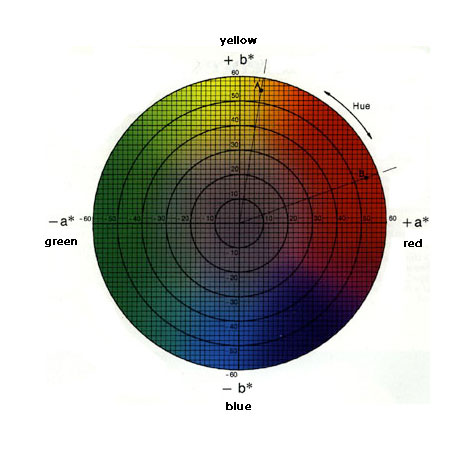
\includegraphics[width=\textwidth]{assets/images/methods/porting/cielab/cielab2.jpg}  
          \caption{Spazio colore CIELAB in 2D}
        \end{minipage}
        \begin{minipage}{0.35\textwidth}
          \centering
          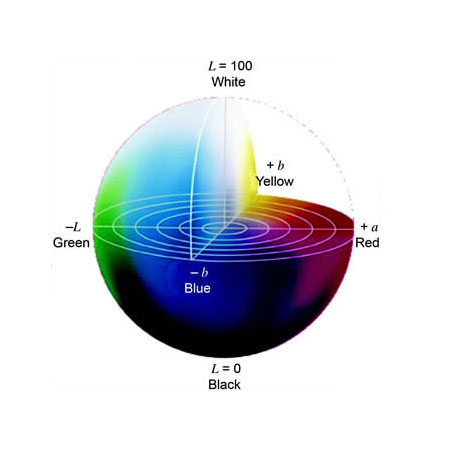
\includegraphics[width=\textwidth]{assets/images/methods/porting/cielab/cielab1.jpg}   
          \caption{Spazio colore CIELAB in 3D}
        \end{minipage}
      \end{figure}

      L'immagine viene convertita nello spazio colore Cielab, è uno spazio \\
      colore-opponente con la dimensione L per la luminosità e a e b per le dimensioni colore-opponente,
      basato sulle coordinate dello spazio colore non lineare compresso CIE XYZ.
      La luminosità è calcolata usando la radice cubica della luminanza relativa. 
      Lab include tutti i colori percepibili, perciò include completamente i gamut degli 
      spazi colore RGB e CMYK ed è indipendente dal dispositivo che li rappresenta.
      
      Come nella versione originale il primo passo è convertire l'immagine da RGB a CIELAB, 
      a differenza di matlab OpenCV utilizza il formato BGR, ovvero il vettore dei colori per ogni pixel è invertito,
      dall'immagine convertita in spazio colore CIELAB si estrae il canale B dall'immagine questo permette di mettere in evidenza 
      le aree blu dell'immagine così da isolare la parte di mare presente nello sfondo delle foto.
      \newpage
      La sogliatura di Otsu, chiamata anche metodo di Otsu, è un algoritmo utilizzato per determinare automaticamente il valore di soglia ottimale per la segmentazione di un'immagine in bianco e nero.
      L'obiettivo della sogliatura è quello di separare i pixel dell'immagine in due classi, generalmente il primo piano (oggetti di interesse) e lo sfondo.
      \begin{figure}
        \centering
        
        \begin{minipage}{0.3\textwidth}
          \centering
          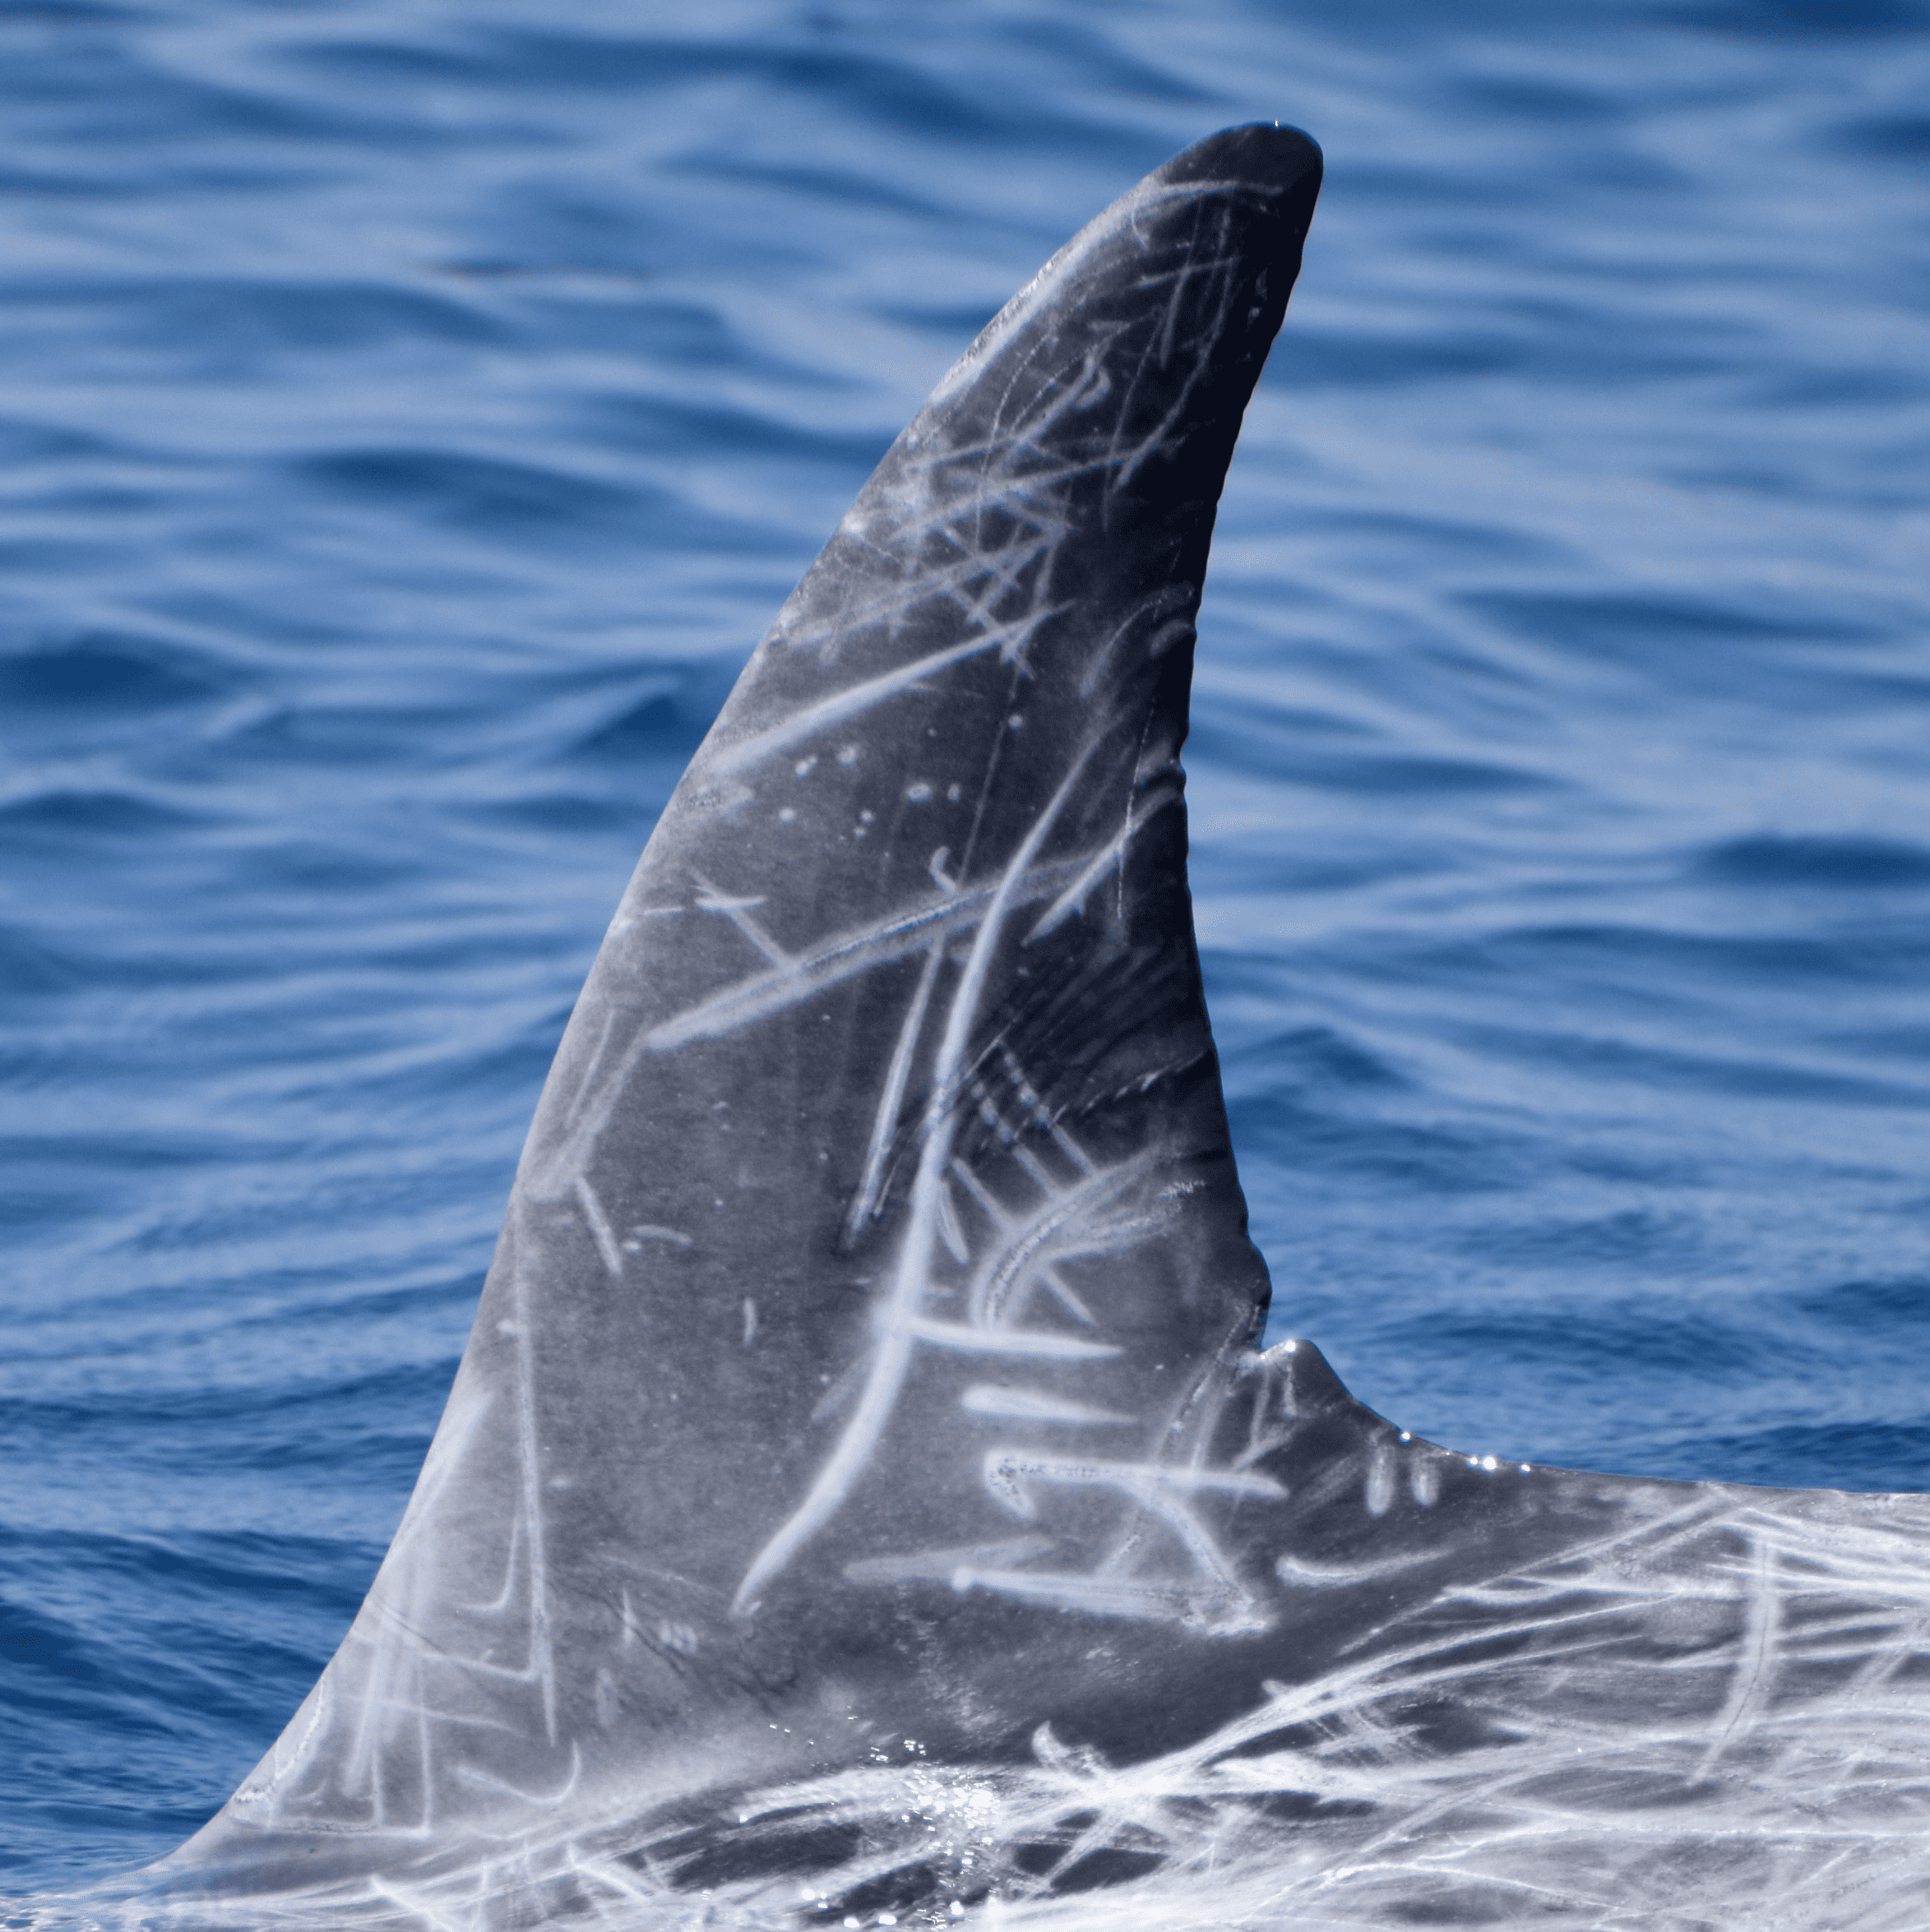
\includegraphics[width=\textwidth]{assets/images/methods/porting/fin_extraction/test_original.png}  
          \caption{Immagine originale}
        \end{minipage}
        \begin{minipage}{0.3\textwidth}
          \centering
          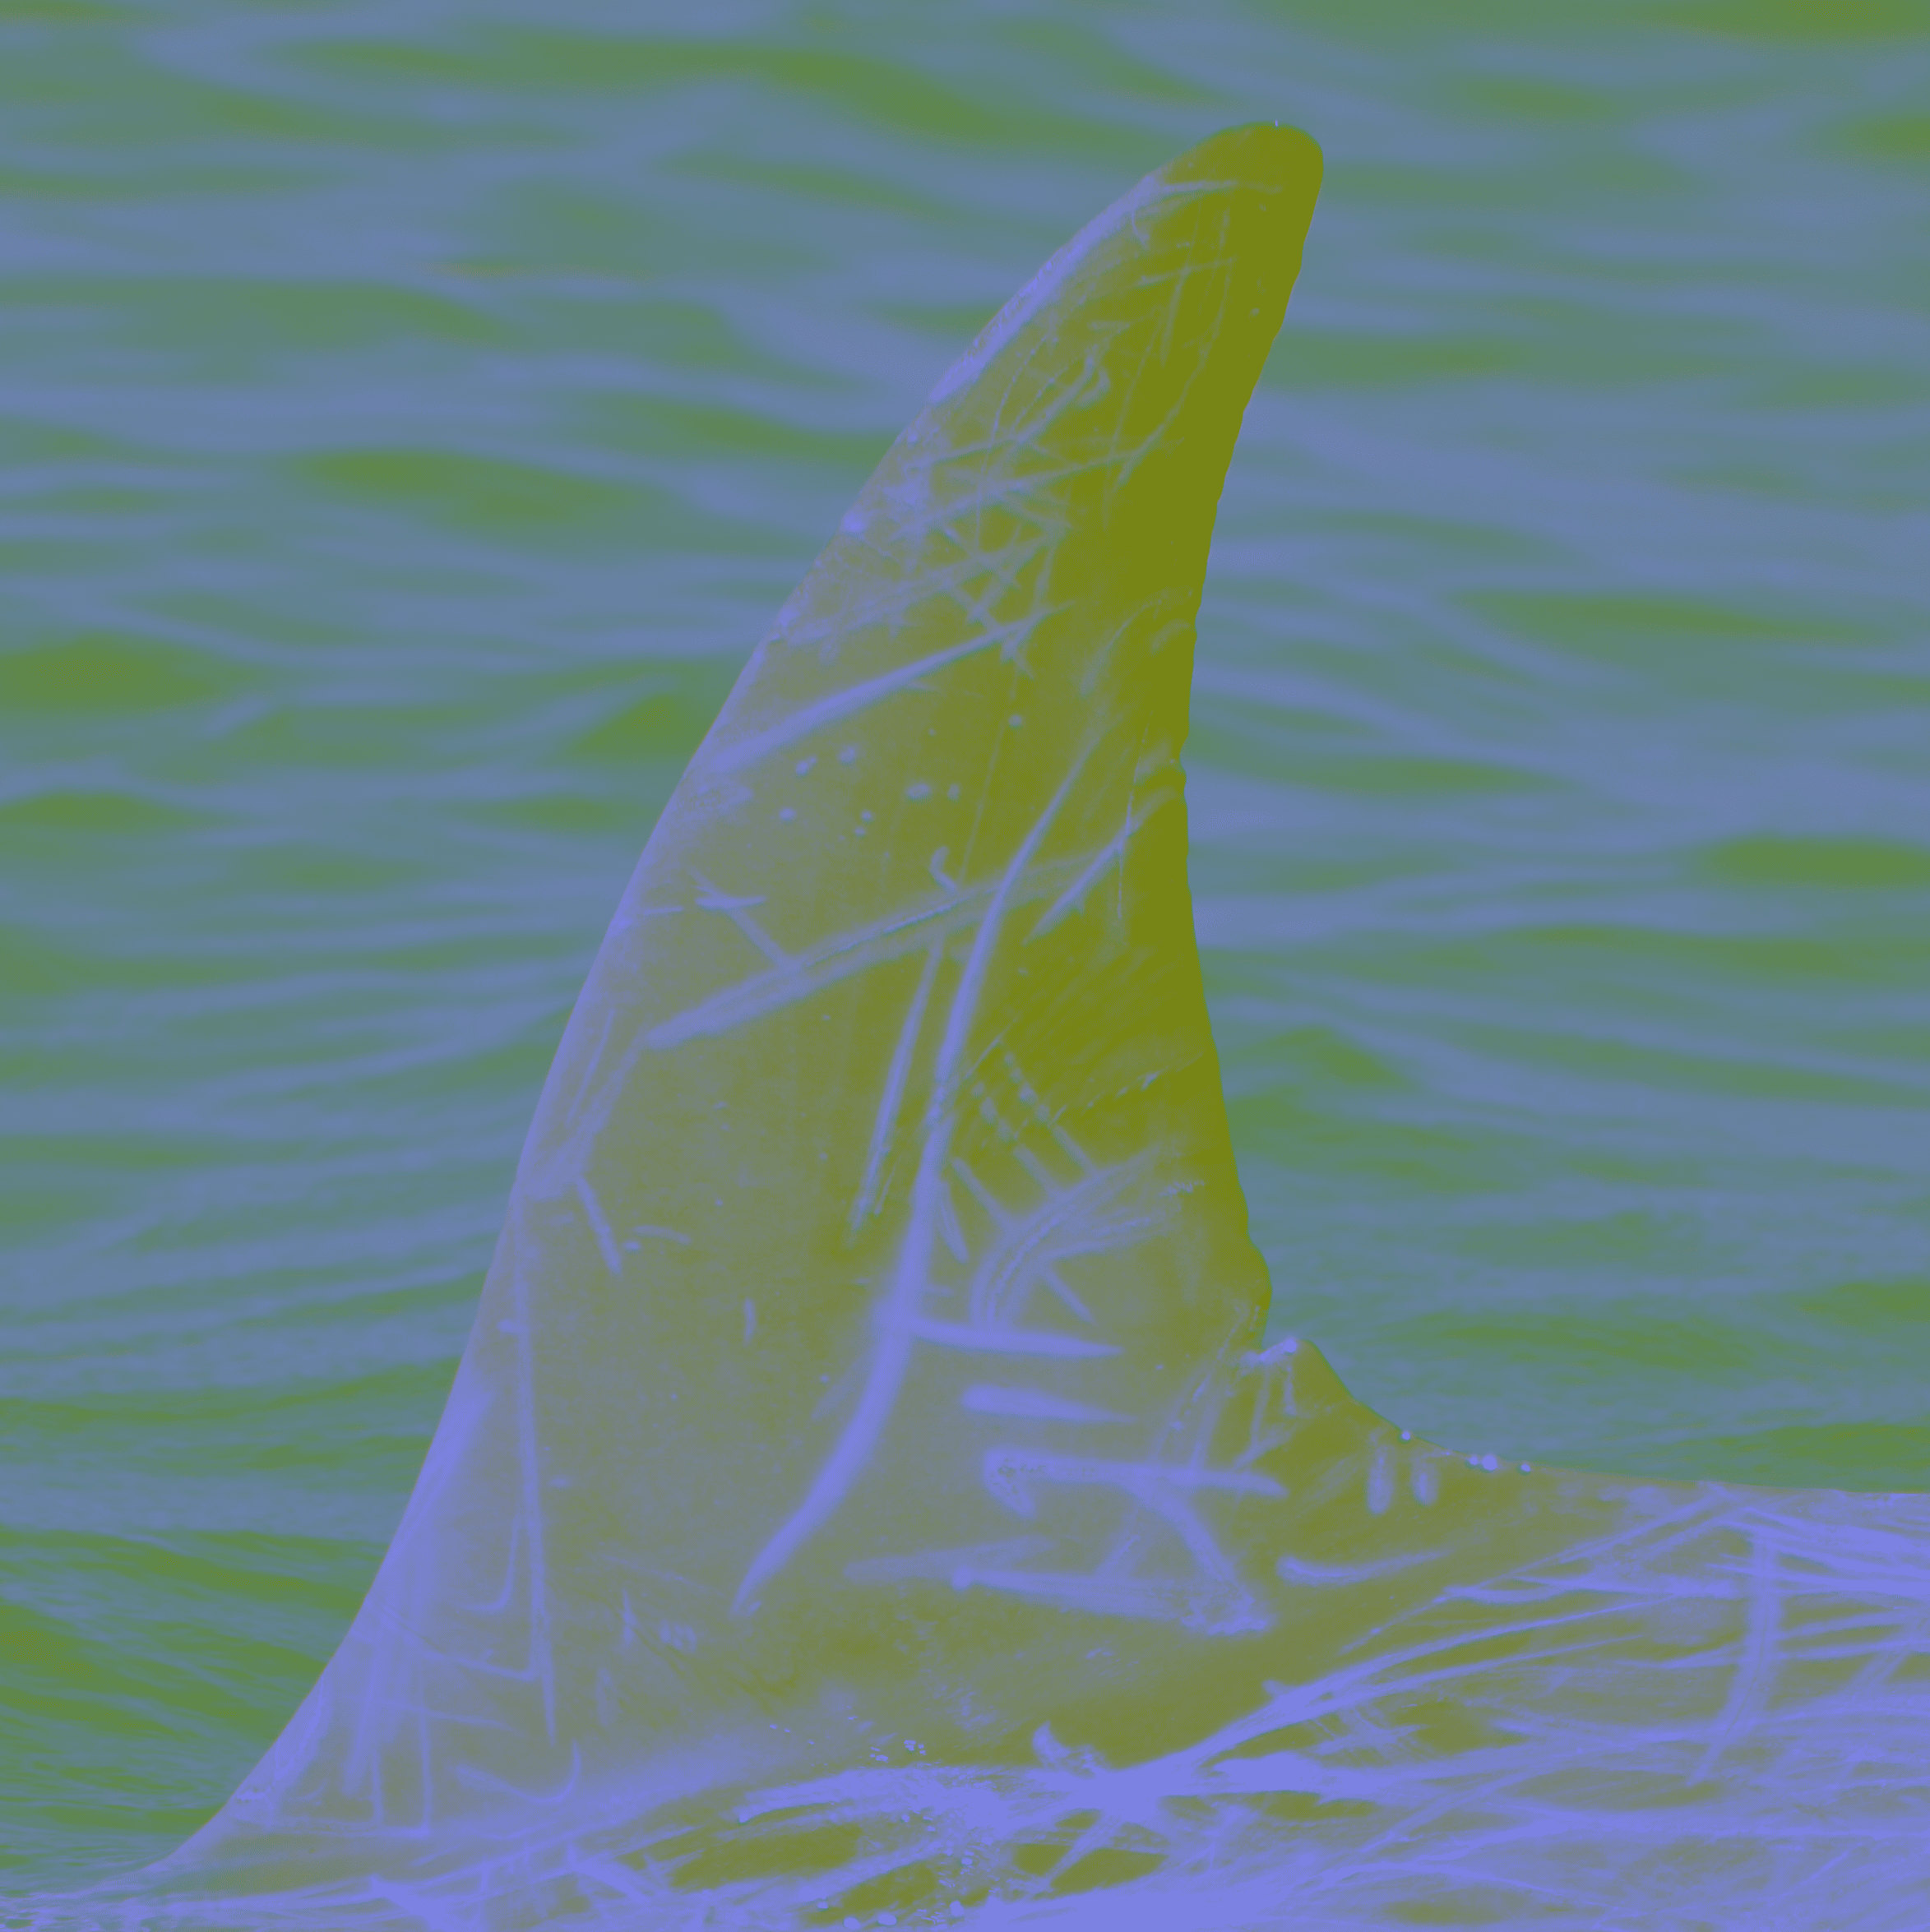
\includegraphics[width=\textwidth]{assets/images/methods/porting/fin_extraction/test_lab.png}   
          \caption{Immagine CIELAB}
        \end{minipage}
        \begin{minipage}{0.3\textwidth}
          \centering
          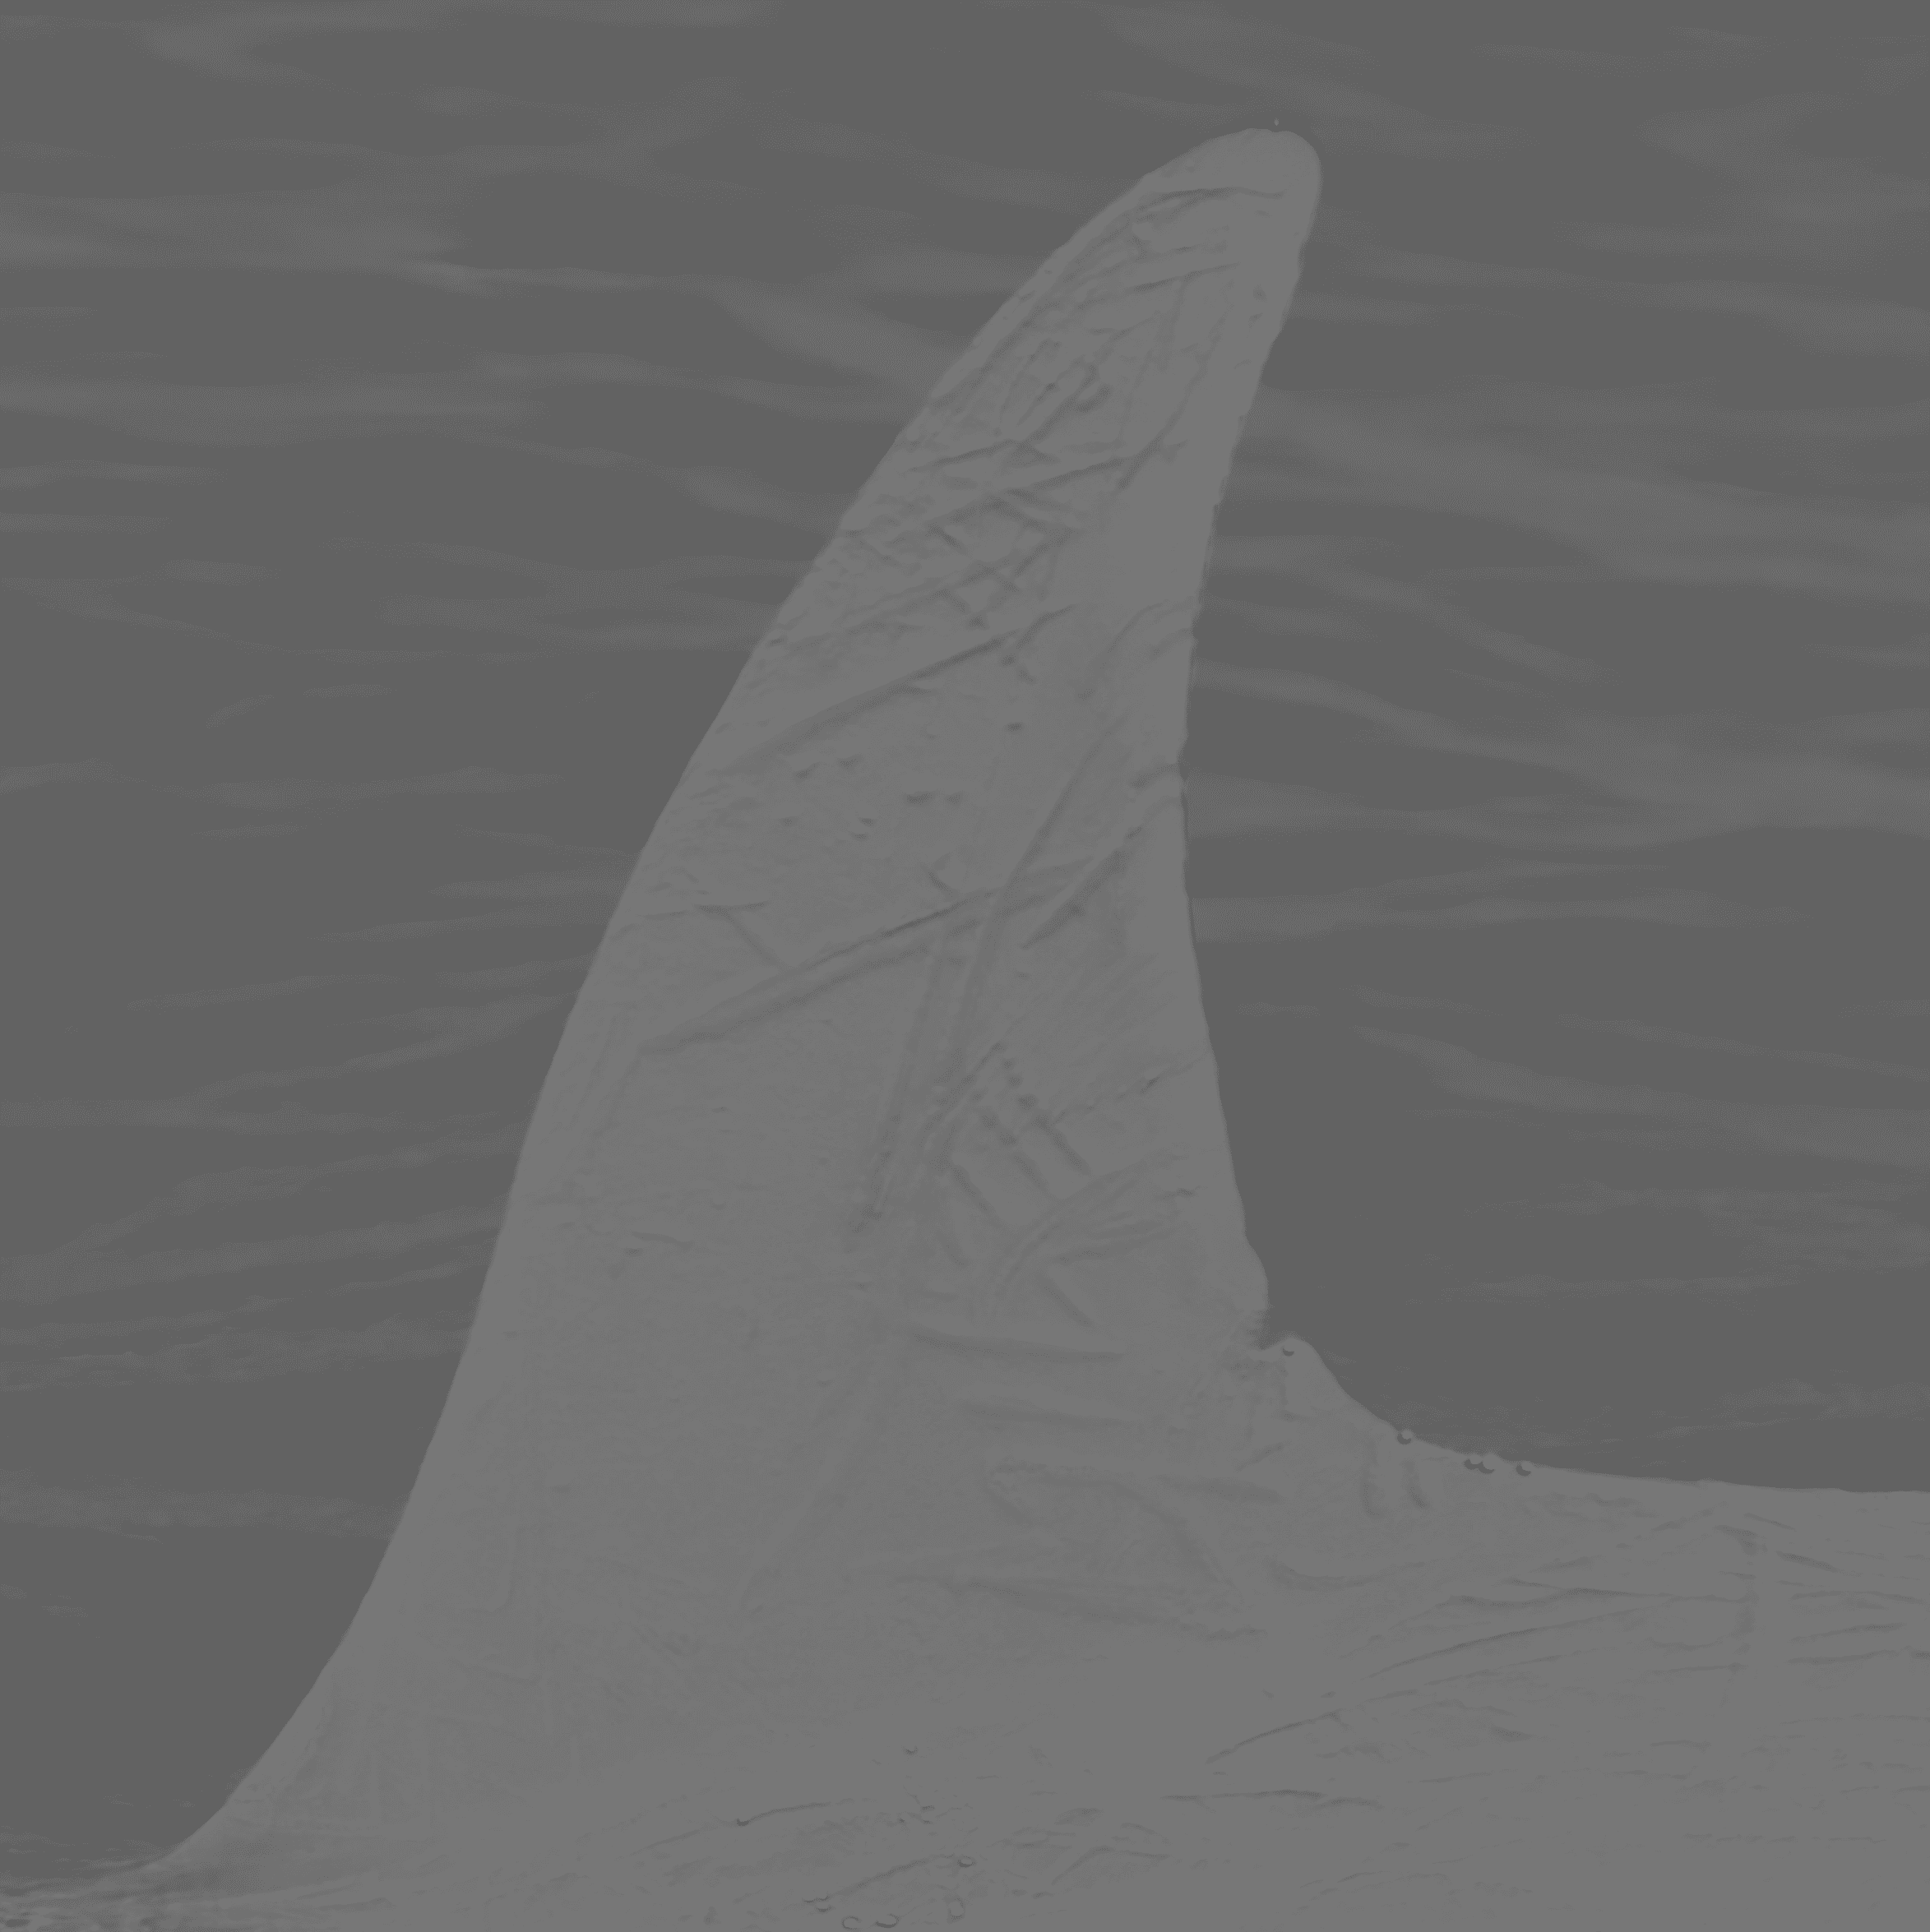
\includegraphics[width=\textwidth]{assets/images/methods/porting/fin_extraction/test_b.png}  
          \caption{Canale B estratto}
        \end{minipage}

        
      \end{figure}

\begin{lstlisting}
#Caricamento immagine originale
image = cv2.imread("BEN_180713_4.png")

#Conversione immagine in spazio colore CIELAB
im_lab = cv2.cvtColor(image, cv2.COLOR_BGR2LAB)

#Estrazione del canale B
b = im_lab[:,:,2]

# Applico il metodo di Otsu al canale B
thr_b, _ = cv2.threshold(b, 0, 255, cv2.THRESH_BINARY + cv2.THRESH_OTSU)
\end{lstlisting}
        L'algoritmo di Otsu \cite{otsu1979threshold} calcola la soglia ottimale in base all'istogramma dei livelli di grigio dell'immagine.
        L'istogramma rappresenta la distribuzione dei valori di grigio presenti nell'immagine.
        \newpage
        L'obiettivo è trovare la soglia che massimizza la varianza tra le due classi (primo piano e sfondo), 
        considerando anche la distribuzione dei pixel di ciascuna classe.
        In altre parole, si cerca la soglia che massimizza la separazione tra i due gruppi di pixel.

      \begin{figure}
        \centering
        \begin{minipage}{0.3\textwidth}
          \centering
          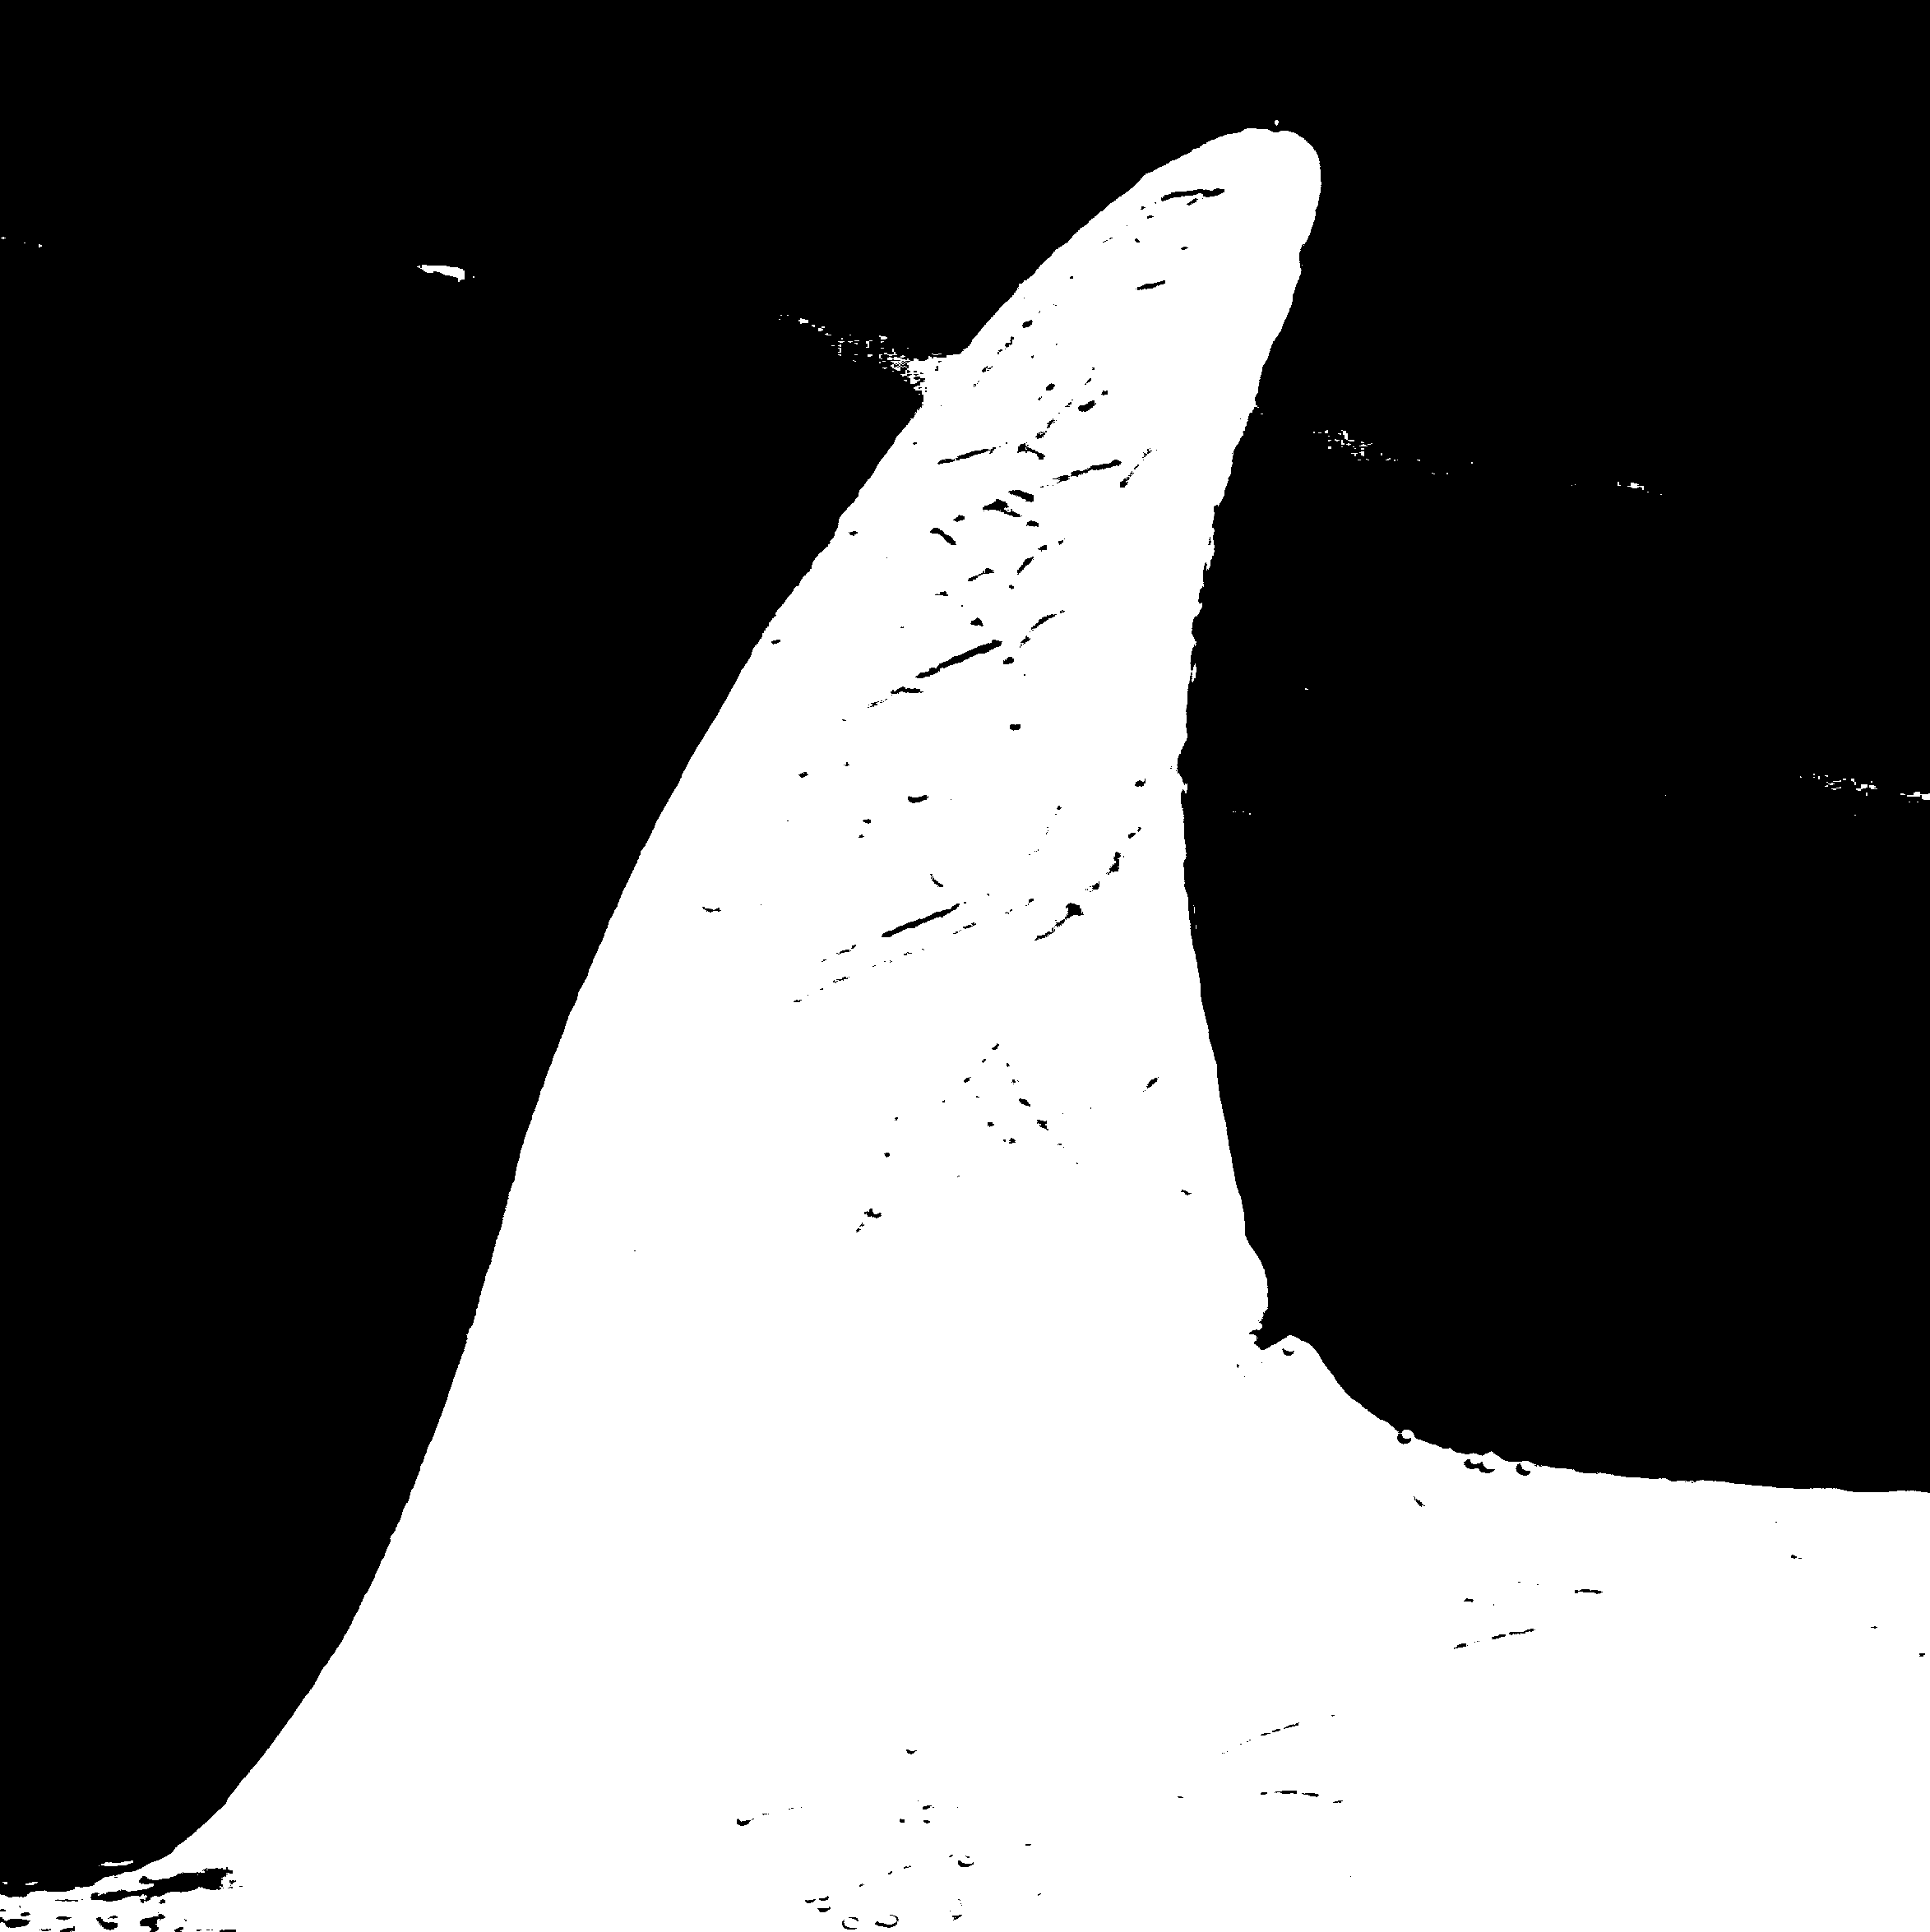
\includegraphics[width=\textwidth]{assets/images/methods/porting/fin_extraction/test_thr_b.png}   
          \caption{Metodo OTSU}
        \end{minipage}
        \begin{minipage}{0.3\textwidth}
          \centering
          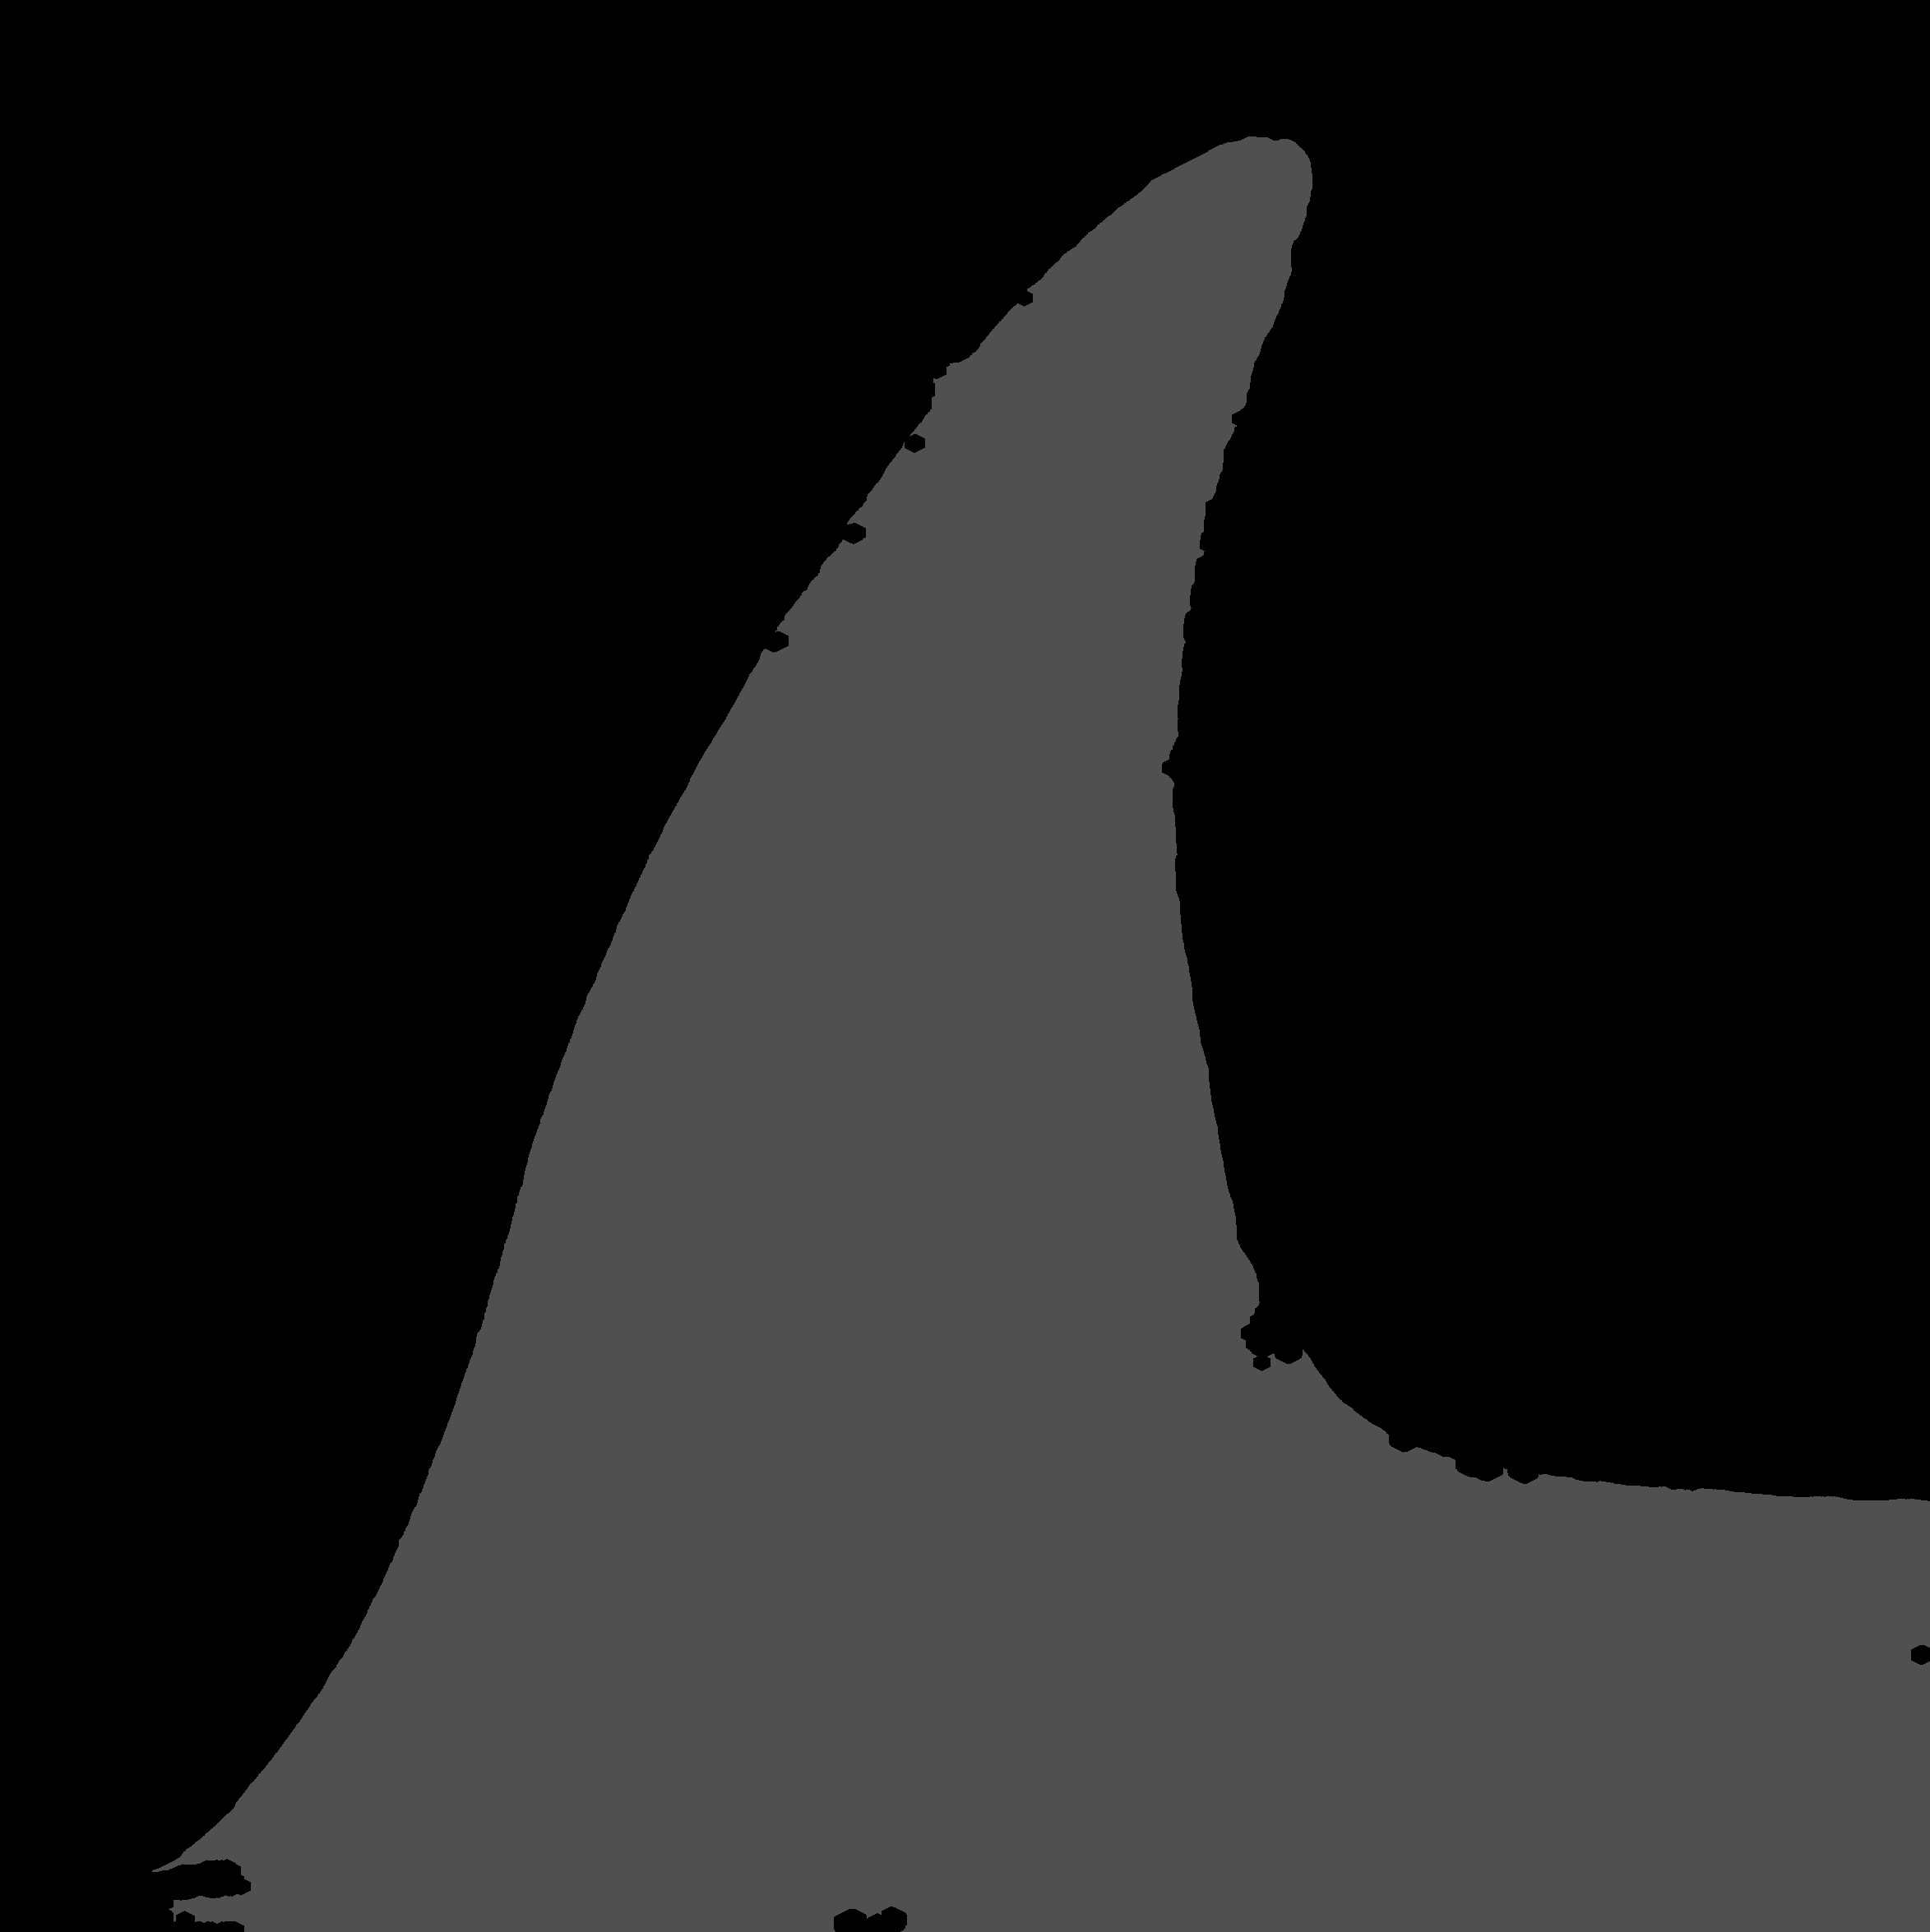
\includegraphics[width=\textwidth]{assets/images/methods/porting/fin_extraction/test_mask1.png}  
          \caption{Operatori morfologici e rimozione segmenti}
        \end{minipage}
        \begin{minipage}{0.3\textwidth}
          \centering
          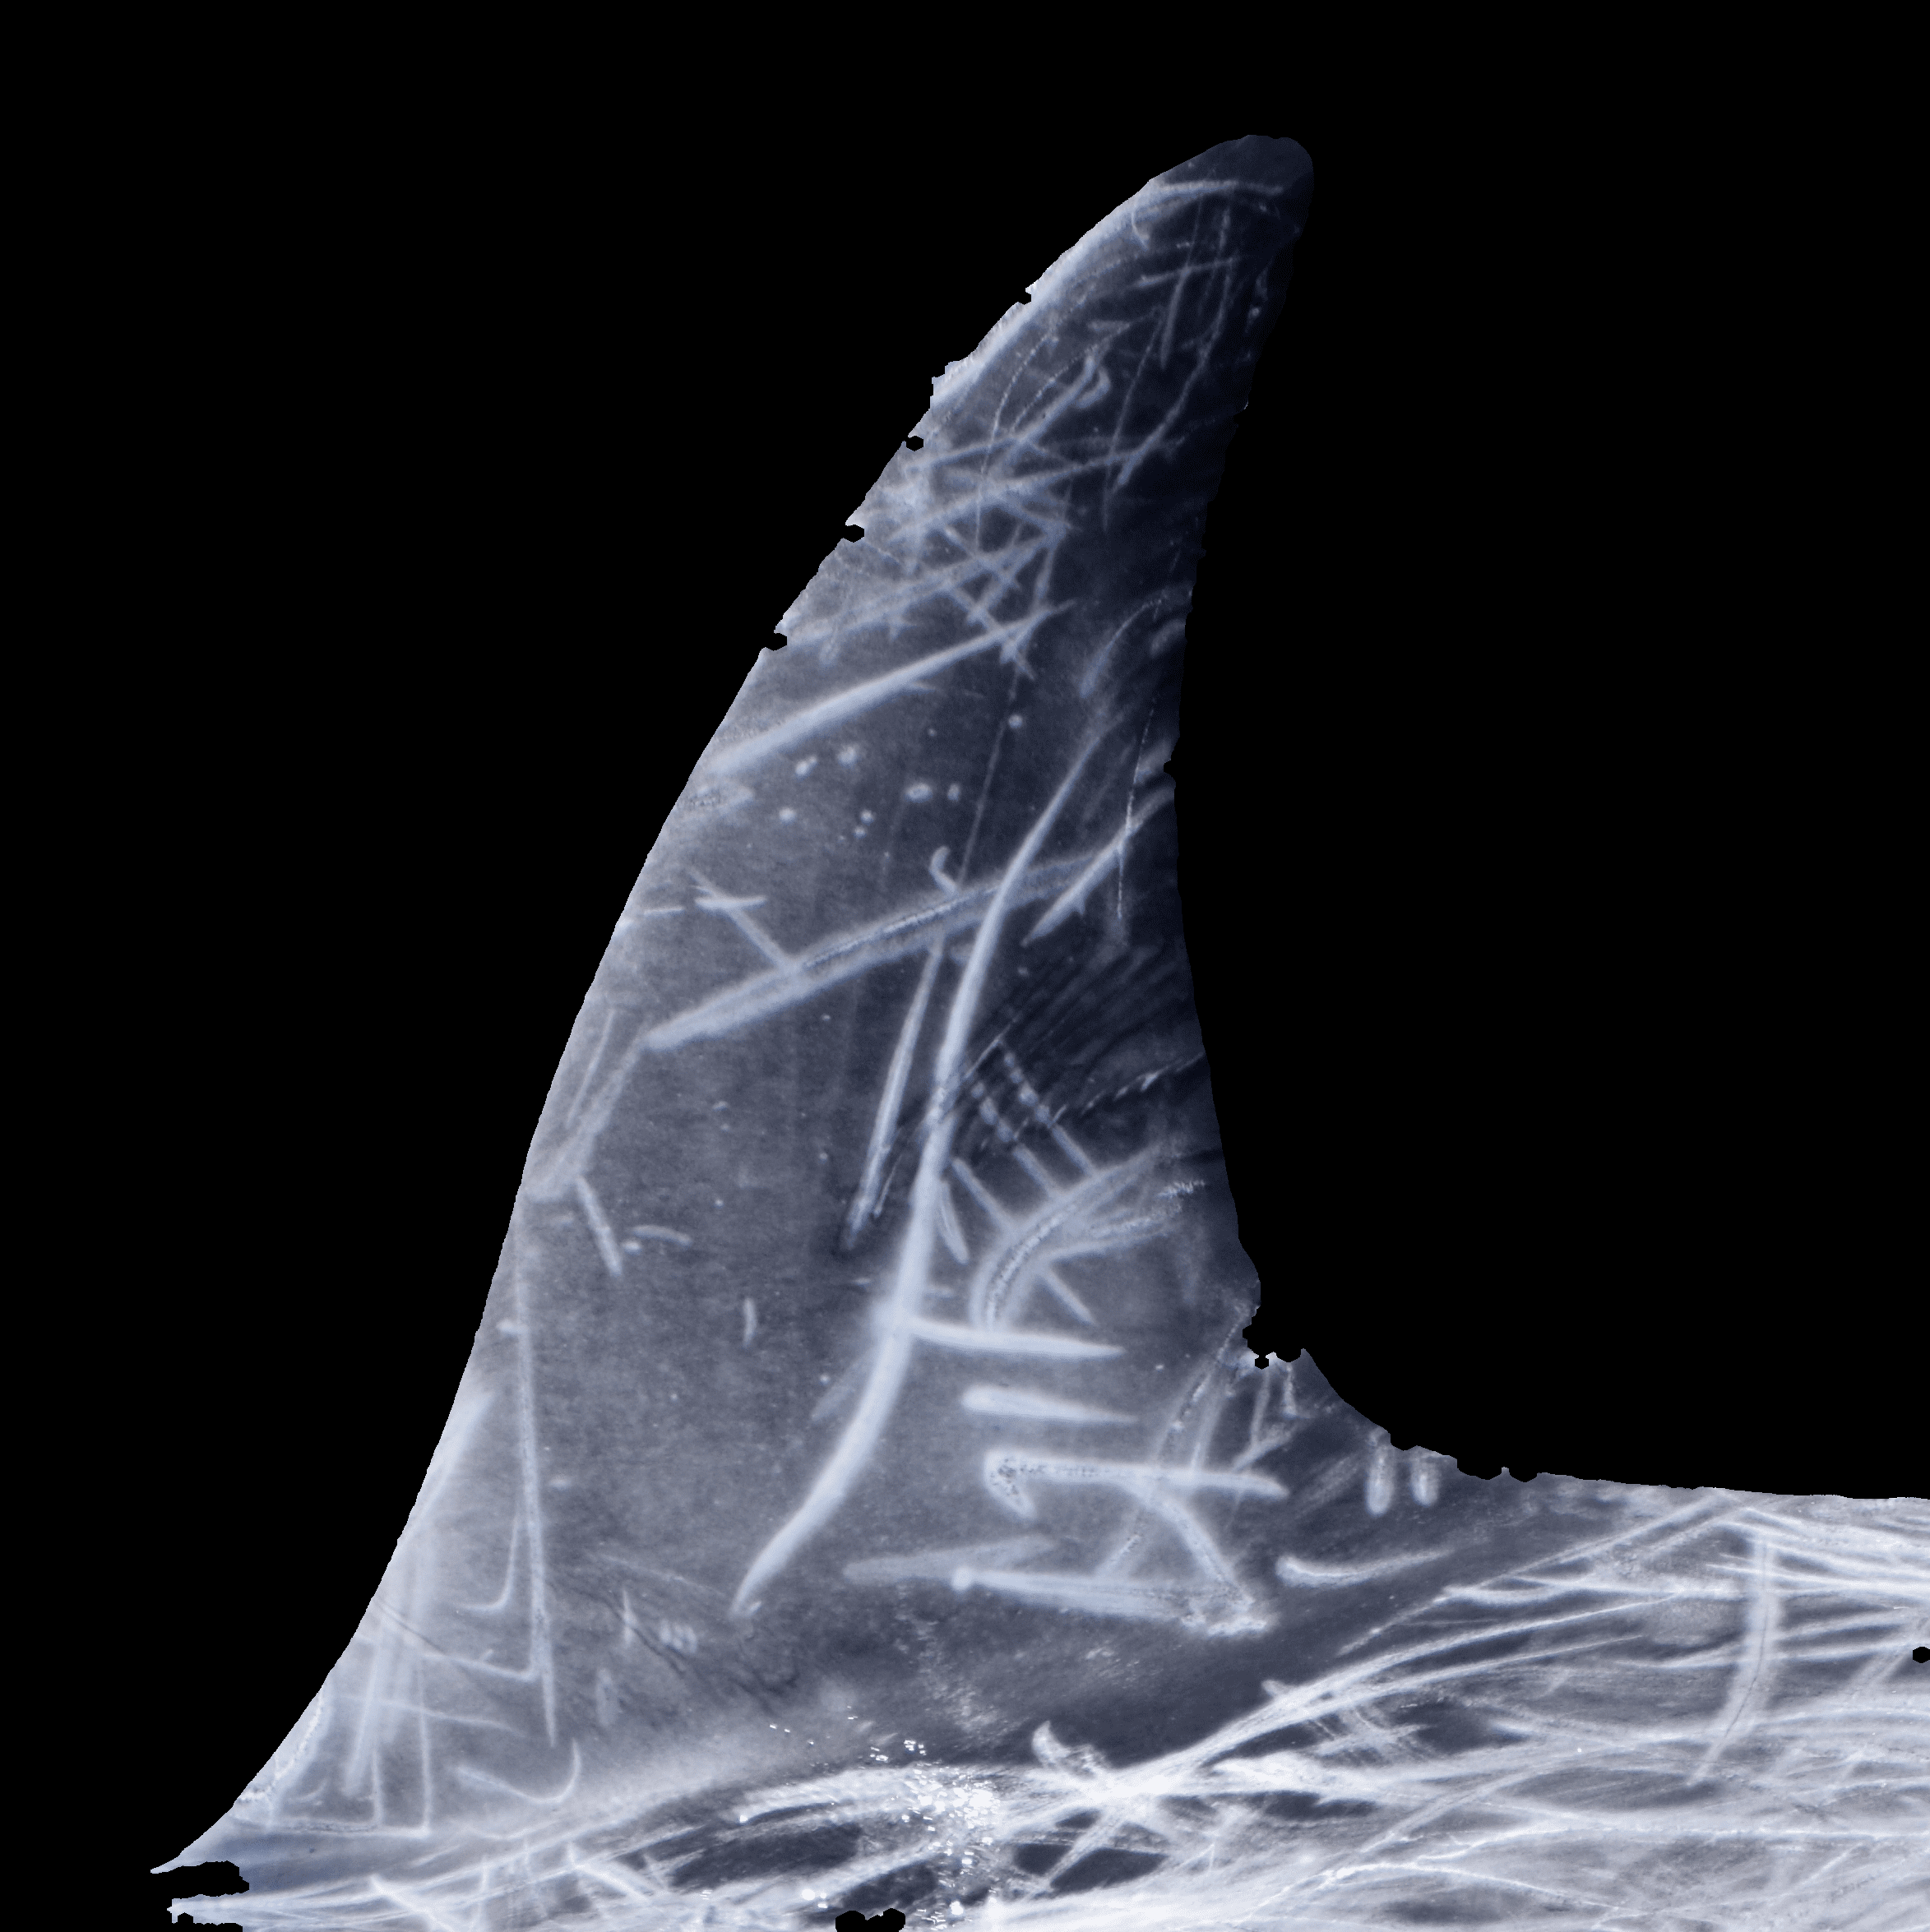
\includegraphics[width=\textwidth]{assets/images/methods/porting/fin_extraction/test_out.png}   
          \caption{Pinna estratta}
        \end{minipage}
        \begin{flushleft}
          
        \end{flushleft}
      \end{figure}
      Una volta prodotta la prima maschera grazie al metodo OTSU, 
      si passa all'eliminazione dei buchi mediante l'utilizzo di operatori
      morfologici e alla rimozione di segmenti slegati dall'area della pinna.
      Nello specifico gli operatori morfologici utilizzati per l'elimiazione dei buchi sono stati:
      \begin{itemize}
        \item Dilatazione (Dilation): L'operazione di dilatazione viene utilizzata per \\espandere le regioni di pixel bianchi nell'immagine. In sostanza, ogni pixel bianco nell'immagine di input viene "gonfiato" e riempito con pixel bianchi circostanti. Ciò ha l'effetto di aumentare le dimensioni dell'oggetto o delle strutture bianche nell'immagine. L'operazione di dilatazione è utile per riempire eventuali buchi o lacune all'interno delle regioni, connettere regioni separate o aumentare la dimensione degli oggetti.
        \newpage
        \item Chiusura (Closing): L'operazione di chiusura combina l'erosione seguita dalla dilatazione per rimuovere piccoli buchi o aree isolate all'interno delle regioni bianche dell'immagine. Inizialmente, l'operazione di erosione viene applicata per ridurre le dimensioni delle regioni bianche e rimuovere dettagli indesiderati. Successivamente, l'operazione di dilatazione viene applicata per riempire i buchi e ricongiungere le regioni vicine che potrebbero essere state separate durante l'erosione. L'operazione di chiusura è utile per ridurre il rumore, migliorare la coerenza delle regioni e completare le forme degli oggetti.
      \end{itemize}
      \begin{figure}[H]
        \centering
        \begin{minipage}{0.3\textwidth}
          \centering
          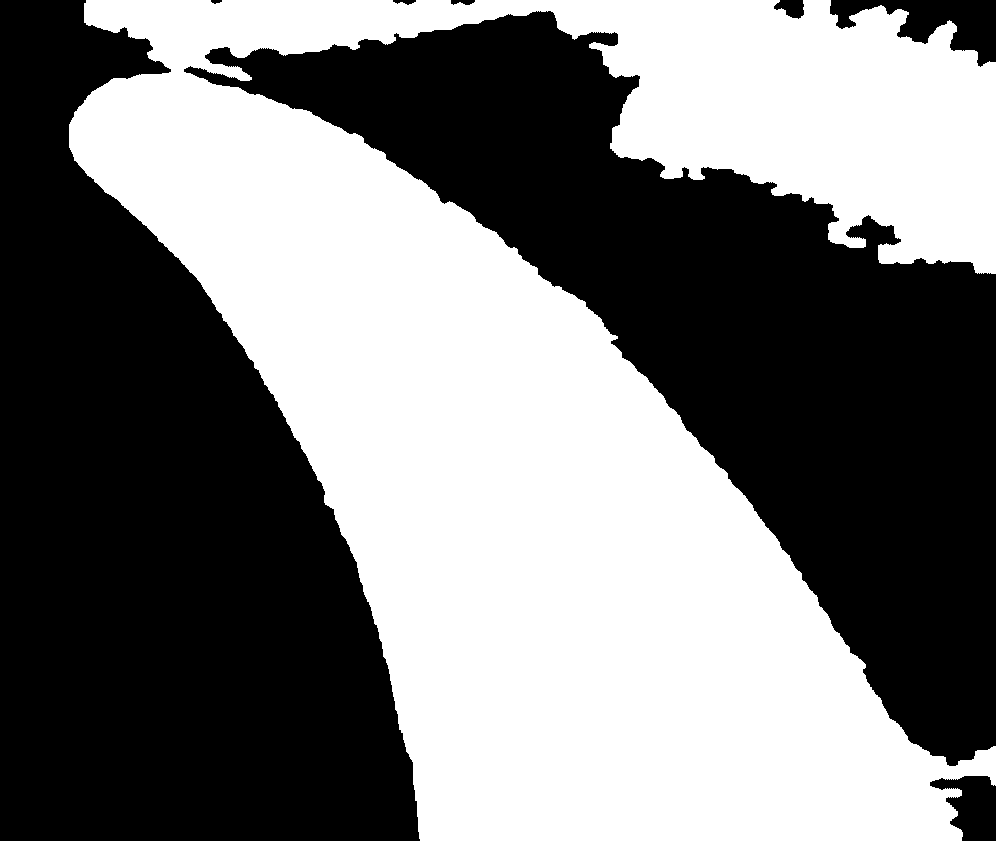
\includegraphics[width=\textwidth]{assets/images/methods/porting/alg_area/original.png}   
          \caption{Maschera originale}
        \end{minipage}
        \begin{minipage}{0.3\textwidth}
          \centering
          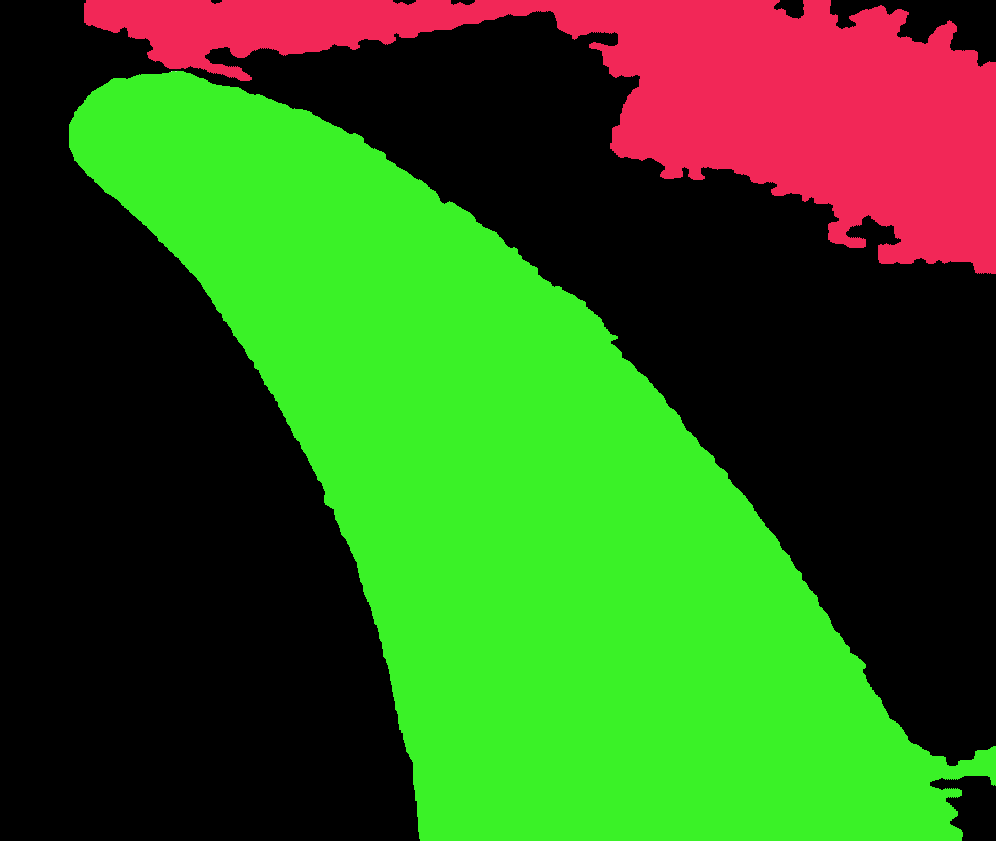
\includegraphics[width=\textwidth]{assets/images/methods/porting/alg_area/find.png}  
          \caption{Divisione in segmenti}
        \end{minipage}
        \begin{minipage}{0.3\textwidth}
          \centering
          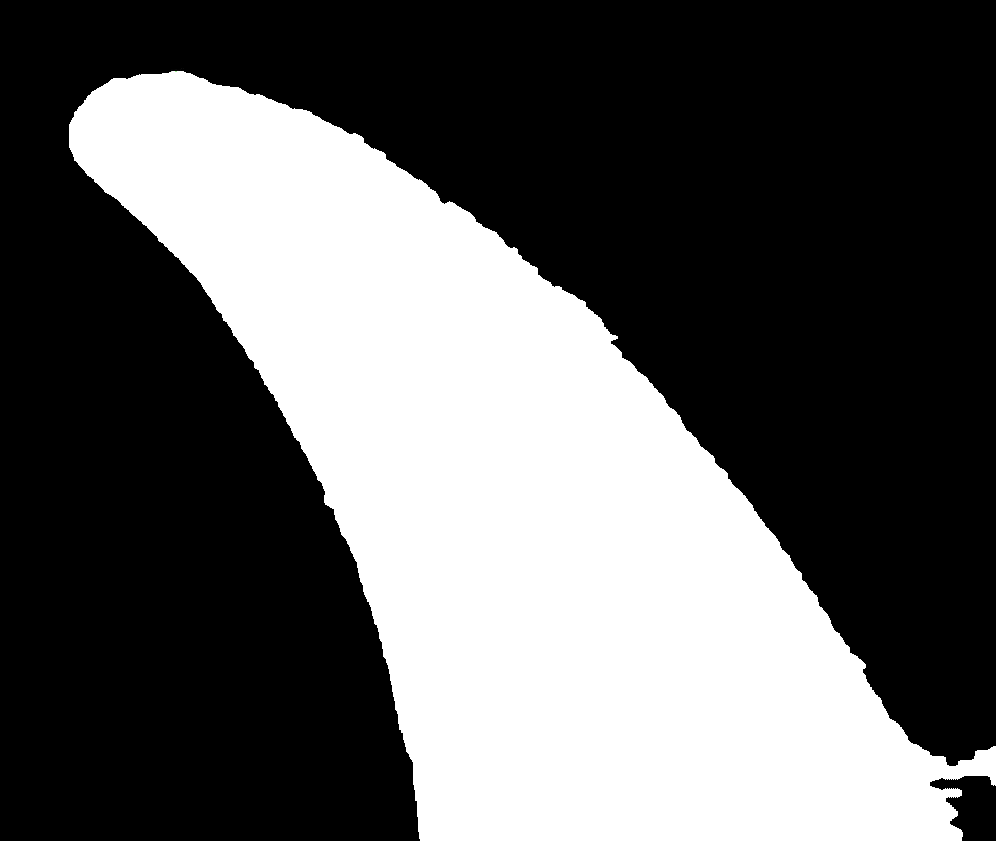
\includegraphics[width=\textwidth]{assets/images/methods/porting/alg_area/clear.png}   
          \caption{Rimozione segmenti minori}
        \end{minipage}
      \end{figure}
     
      Per quanto riguarda l'eliminazione di segmenti non appartenenti all'area della pinna del delfino
      è stato scritto un algoritmo che si basa sul trovare tutti i segmenti separati all'interno della maschera,
      cercare quello con l'area maggiore e poi rimuovere tutto il resto dalla maschera, 
      questa operazione viene ripetuta sia prima che dopo l'utilizzo degli operatori morfologici, con il fine di
      eliminare eventuali scarti dell'erosione o del metodo OTSU.
      \newpage

\begin{lstlisting}
#Trova i contorni nella maschera
contours, _ = cv2.findContours(im_thr, cv2.RETR_TREE, cv2.CHAIN_APPROX_NONE)

biggest_area = -1;
biggest = None;

for contour in contours:
    #Viene calcolata l'area del contorno
    area = cv2.contourArea(contour);

    #Salvataggio del contorno con l'area maggiore
    if biggest_area < area:
        biggest_area = area;
        biggest = contour;

#Disegno la maschera del contorno maggiore sulla maschera originale con una tonalità di grigio diversa
mask_colored = cv2.drawContours(im_thr, [biggest], -1, 80, -1);
_, binary_image = cv2.threshold(mask_colored, 254, 255, cv2.THRESH_BINARY_INV)

#Estraggo la maschera del contorno maggiore
mask = cv2.bitwise_and(mask_colored, mask_colored, mask=binary_image)

kernel = cv2.getStructuringElement(cv2.MORPH_ELLIPSE, (5,5))

#Applico operatori morfologici per eliminare eventuali buchi nella maschera
mask = cv2.morphologyEx(mask, cv2.MORPH_DILATE, kernel=kernel, iterations=1)
mask = cv2.morphologyEx(mask, cv2.MORPH_CLOSE, kernel=kernel, iterations=1)

#Altra Rimozione dei segmenti
#...
#Applico la maschera all'immagine originale per estrarre la pinna
fin = cv2.bitwise_and(image, image, mask=mask)
\end{lstlisting}
    \subsection{Controllo qualità}
    \begin{figure}[H]
      \centering
      \begin{minipage}{0.3\textwidth}
        \centering
        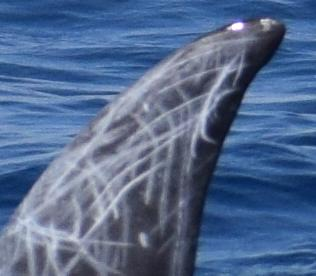
\includegraphics[width=\textwidth]{assets/images/methods/porting/quality_control/blur.png}  
        \caption{Foto sfocata (Blur)}
      \end{minipage}
      \begin{minipage}{0.3\textwidth}
        \centering
        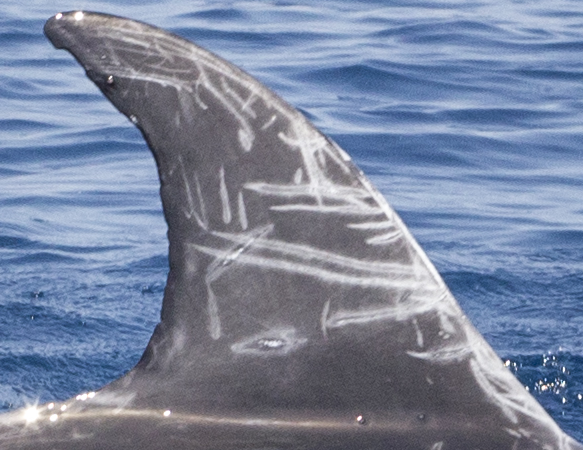
\includegraphics[width=\textwidth]{assets/images/methods/porting/quality_control/contrast.png}   
        \caption{Foto con basso contrasto (Contrast)}
      \end{minipage}
      \begin{minipage}{0.3\textwidth}
        \centering
        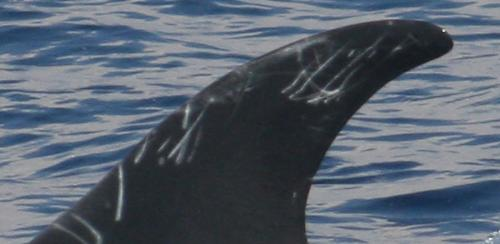
\includegraphics[width=\textwidth]{assets/images/methods/porting/quality_control/snr.png}   
        \caption{Foto con rumore (SNR)}
      \end{minipage}
    \end{figure}
    Una prima fase di filtraggio delle immagini viene applicata utilizzando dei metodi di 
    controllo della qualità delle immagini, questo con il fine di scartare le foto con caratteristiche 
    che andrebbero a compromettere a priori la fase di estrazione della maschera, data la scarsa qualità,
    per effettuare questo controllo di utilizzano le seguenti metriche:
    \begin{itemize}
      \item Blur (sfocatura): La sfocatura si riferisce alla mancanza di nitidezza o di dettaglio nell'immagine. Misurare il livello di sfocatura è importante per valutare la qualità e la definizione di un'immagine. La sfocatura può essere causata da vari fattori come l'acquisizione non precisa dell'immagine, il movimento della fotocamera durante lo scatto o la compressione dell'immagine. La metrica di blur viene utilizzata per quantificare il grado di sfocatura presente nell'immagine e può aiutare a determinare se l'immagine soddisfa i requisiti desiderati in termini di nitidezza.
      \begin{lstlisting}
#Calcola la sfocatura utlizzando
#il filtro Laplaciano
blur = cv2.Laplacian(fin_gray, cv2.CV_64F).var()
      \end{lstlisting}
   
      \newpage
      \item Contrast (contrasto): Il contrasto si riferisce alla differenza di luminosità tra le diverse parti di un'immagine. Un buon contrasto è importante perché consente di distinguere meglio gli oggetti e i dettagli presenti nell'immagine. La metrica di contrasto valuta la differenza di intensità tra le regioni chiare e quelle scure dell'immagine. Un contrasto adeguato può migliorare la leggibilità e l'interpretazione dell'immagine stessa.
      \begin{lstlisting}
#Calcola il contrasto 
#utilizzando la deviazione standard
contrast = np.std(fin_gray)
      \end{lstlisting}
      \item SNR (Signal-to-Noise Ratio) o rapporto segnale-rumore: L'SNR è una misura che indica il livello del segnale rispetto al rumore presente in un'immagine. Il rumore può essere causato da vari fattori come l'acquisizione dell'immagine con condizioni di illuminazione scarsa, l'interferenza elettrica o il rumore introdotto durante la trasmissione o la compressione dell'immagine. Un alto rapporto segnale-rumore indica che il segnale (informazione utile) è predominante rispetto al rumore indesiderato nell'immagine. L'SNR è una metrica importante per valutare la qualità e la fedeltà dell'immagine, in quanto un alto SNR indica una migliore qualità dell'immagine in termini di dettaglio e fedeltà visiva.
      \begin{lstlisting}
signal_energy = np.sum(fin_gray ** 2)
noise_energy = np.sum((fin_gray - cv2.GaussianBlur(fin_gray, (5, 5), 0)) ** 2)
snr = 10 * np.log10(signal_energy / noise_energy)
      \end{lstlisting}
    \end{itemize}


    \begin{figure}[H]
      \centering
      \begin{minipage}{0.4\textwidth}
        \centering
        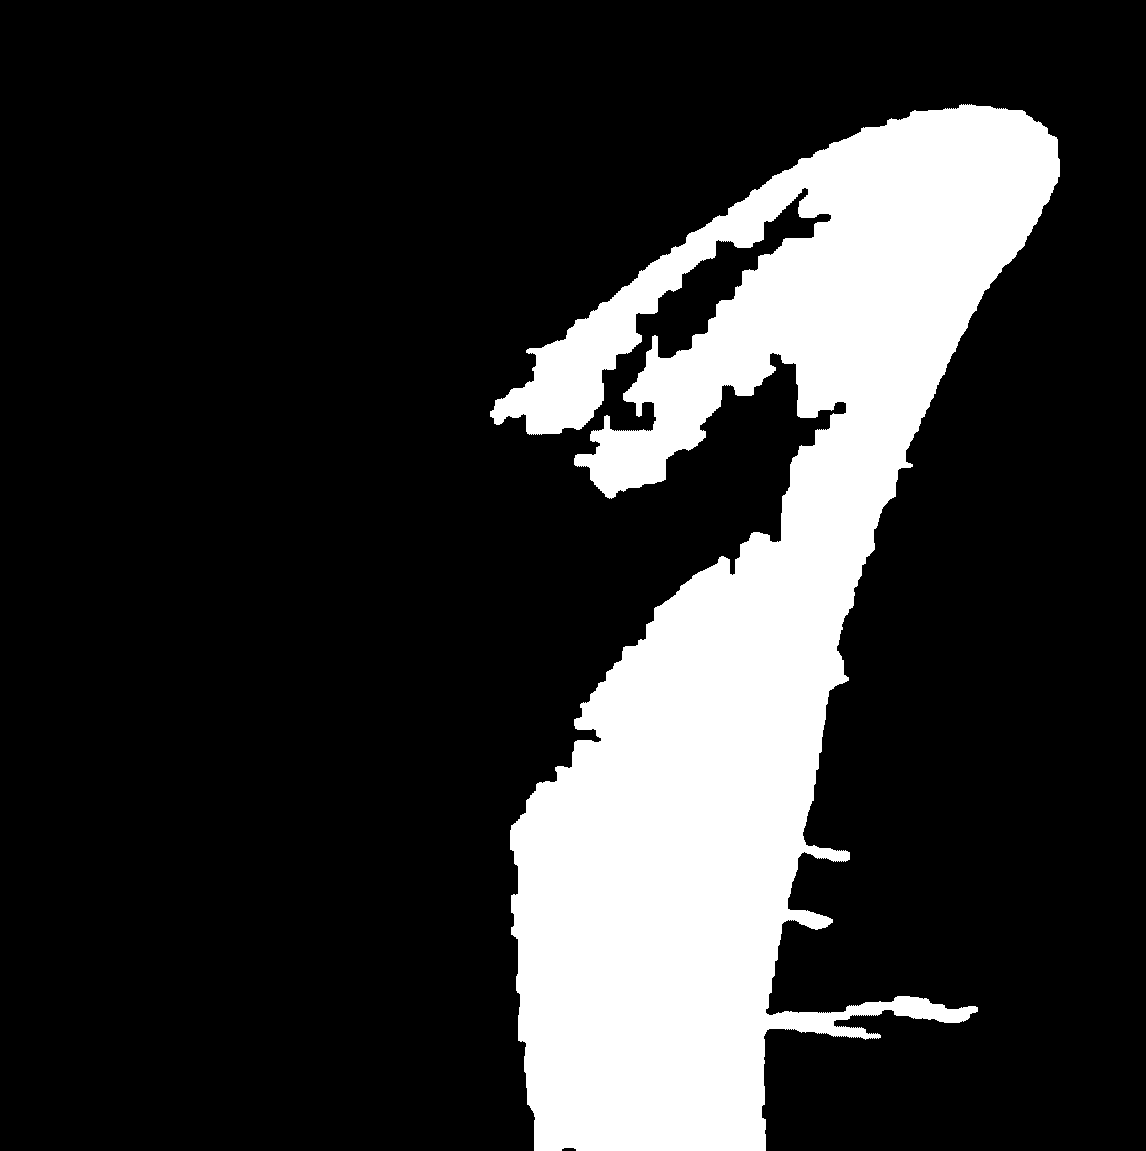
\includegraphics[width=\textwidth]{assets/images/methods/porting/quality_control/less.png}  
        \caption{\\$finArea < minFinArea$}
      \end{minipage}
      \begin{minipage}{0.4\textwidth}
        \centering
        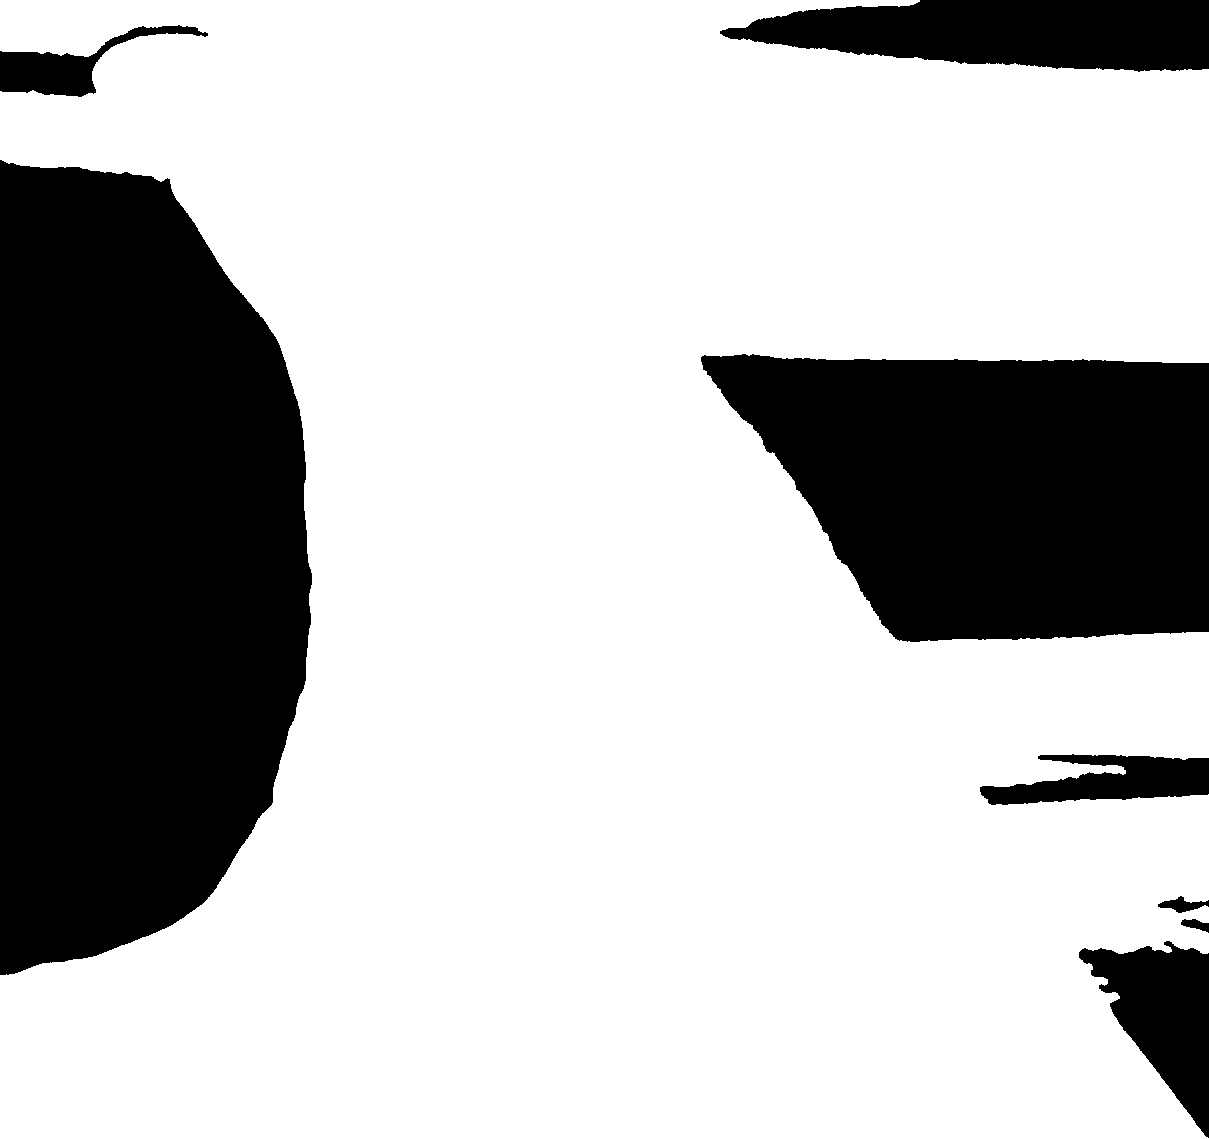
\includegraphics[width=\textwidth]{assets/images/methods/porting/quality_control/too.png}   
        \caption{\\$maxFinArea < finArea$}
      \end{minipage}
    \end{figure}
    Per migliorare la qualità complessiva delle pinne estratte da passare alla fase di feature extraction,
    si sceglie di porre diversi livelli di filtraggio con relativi parametri soglia,
    un controllo viene effetuato sulla maschera generata, ovvero, se 
    dopo tutti i passaggi di ottimizzazione della maschera (compresa l'eliminazione di
    segmenti), l'area della maschera non rispetta la seguente disequazione:
    \begin{minipage}{1\textwidth}
      \centering
      $minFinArea \leq finArea \leq maxFinArea$
    \end{minipage}
    
    Allora l'immagine sarà scartata, dato che sicuramente l'estrazione della maschera
    non avrà correttamente segmentato la pinna del delfino, sia in caso di eccesso o assenza di area.
    
    \begin{lstlisting}
min_fin_area = 33, max_fin_area = 66
mask_pixels = np.sum(mask == 255)
total_pixels = mask.shape[0] * mask.shape[1]
fin_area = (mask_pixels / total_pixels)*100
# ...
if fin_area < min_fin_area or fin_area > max_fin_area:
  model.state = ModelData.ERR_AREA
  return model

model.state = ModelData.OK
return model
    \end{lstlisting}
    \newpage
   
    \subsection{Estrazione feature}
    \begin{figure}[H]
      
      \centering
      \begin{minipage}{0.3\textwidth}
        \centering
        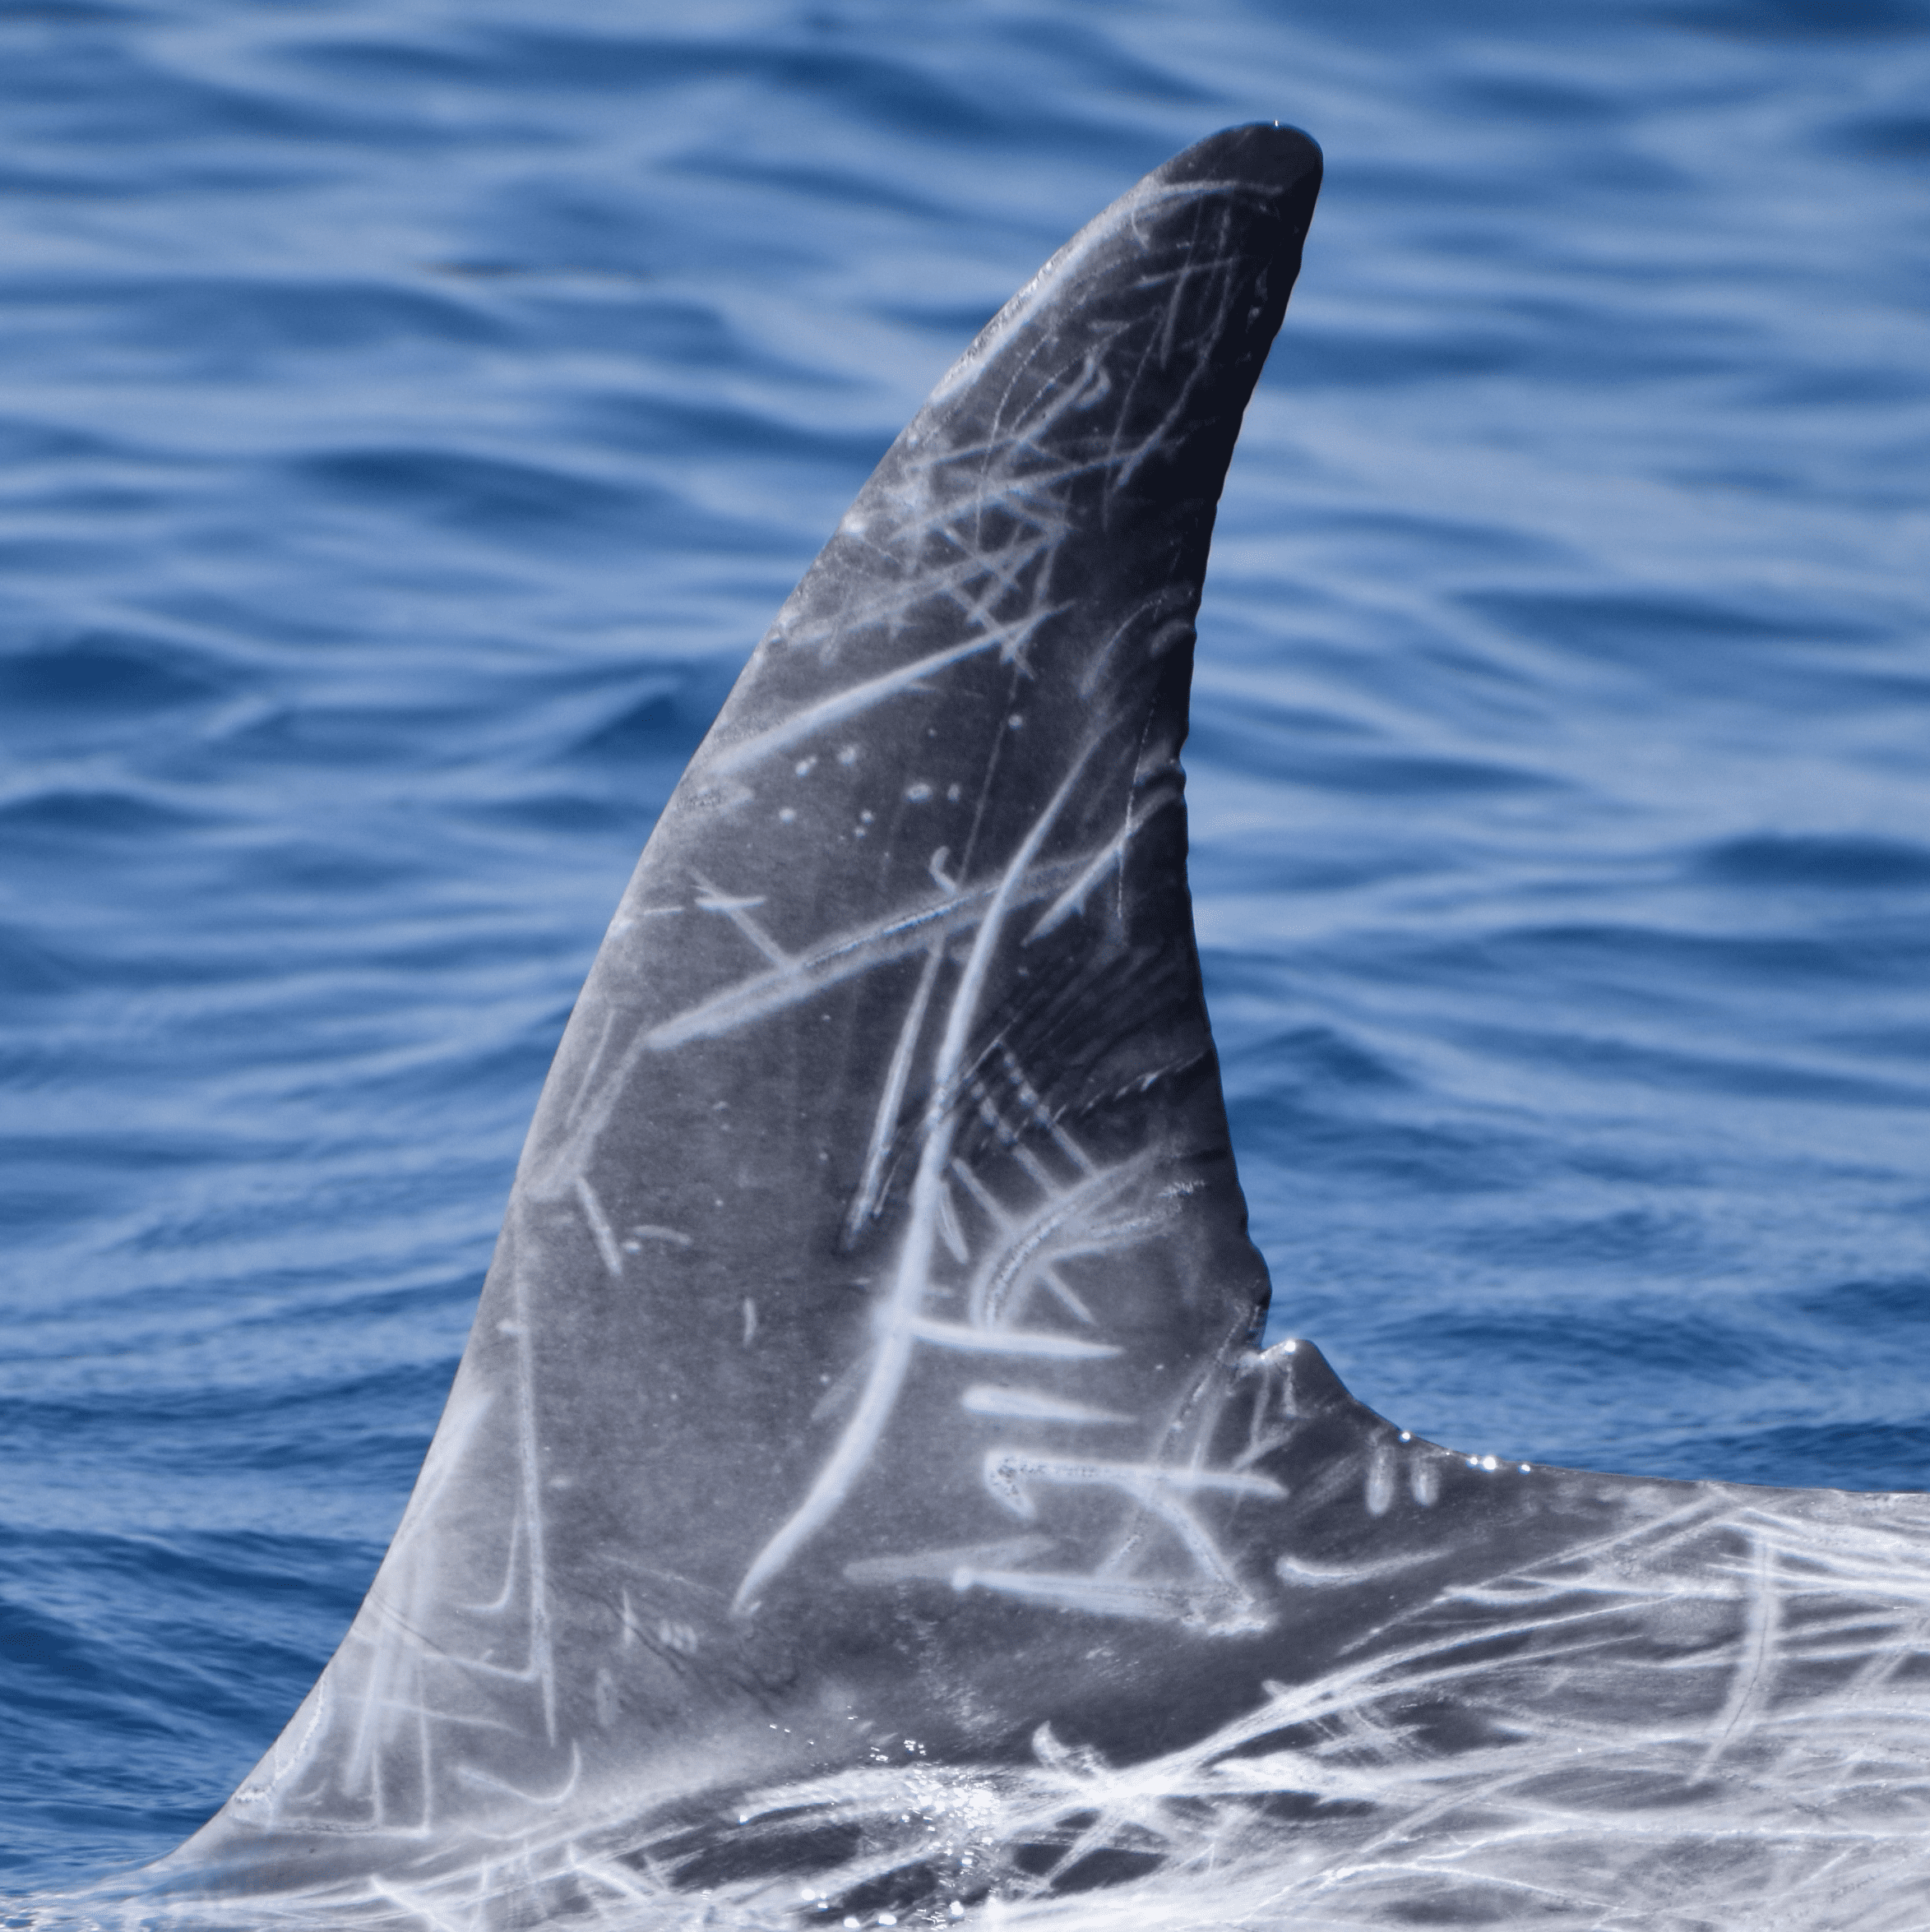
\includegraphics[width=\textwidth]{assets/images/methods/porting/features_extraction/original.png}   
        \caption{Immagine originale}
      \end{minipage}
      \begin{minipage}{0.3\textwidth}
        \centering
        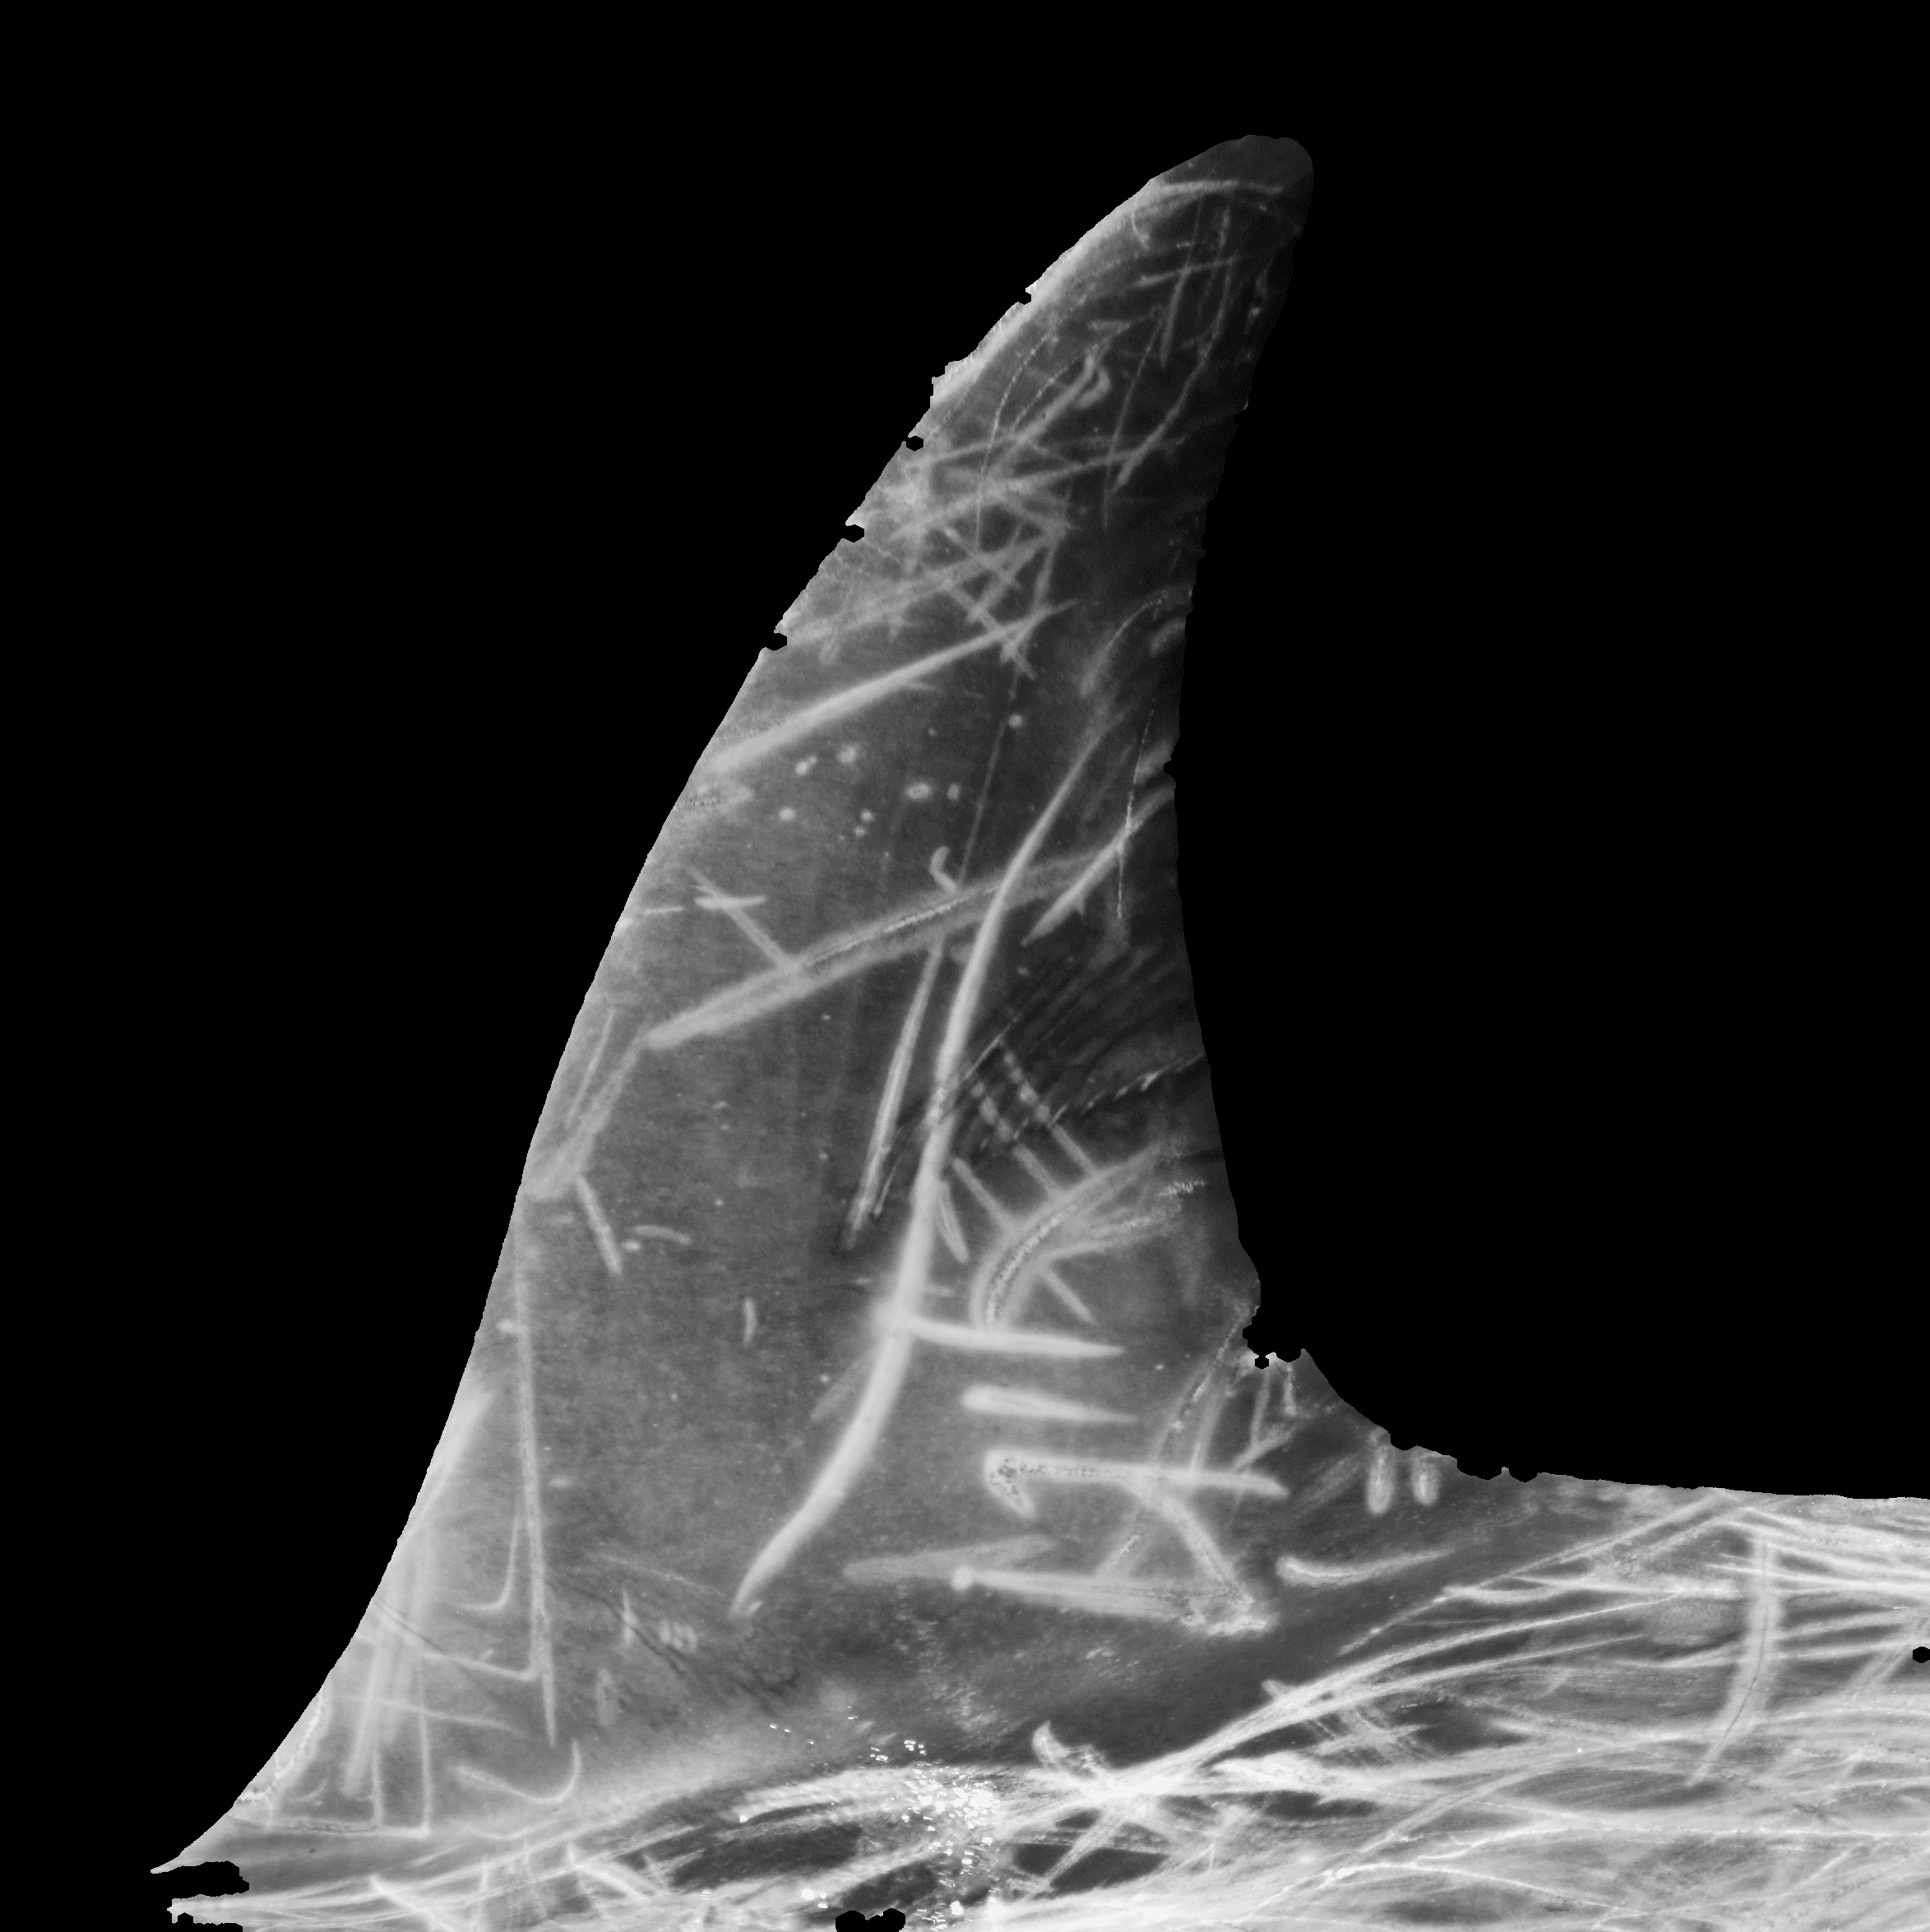
\includegraphics[width=\textwidth]{assets/images/methods/porting/features_extraction/gray.png}  
        \caption{Pinna estratta in scala di grigi}
      \end{minipage}
      \begin{minipage}{0.3\textwidth}
        \centering
        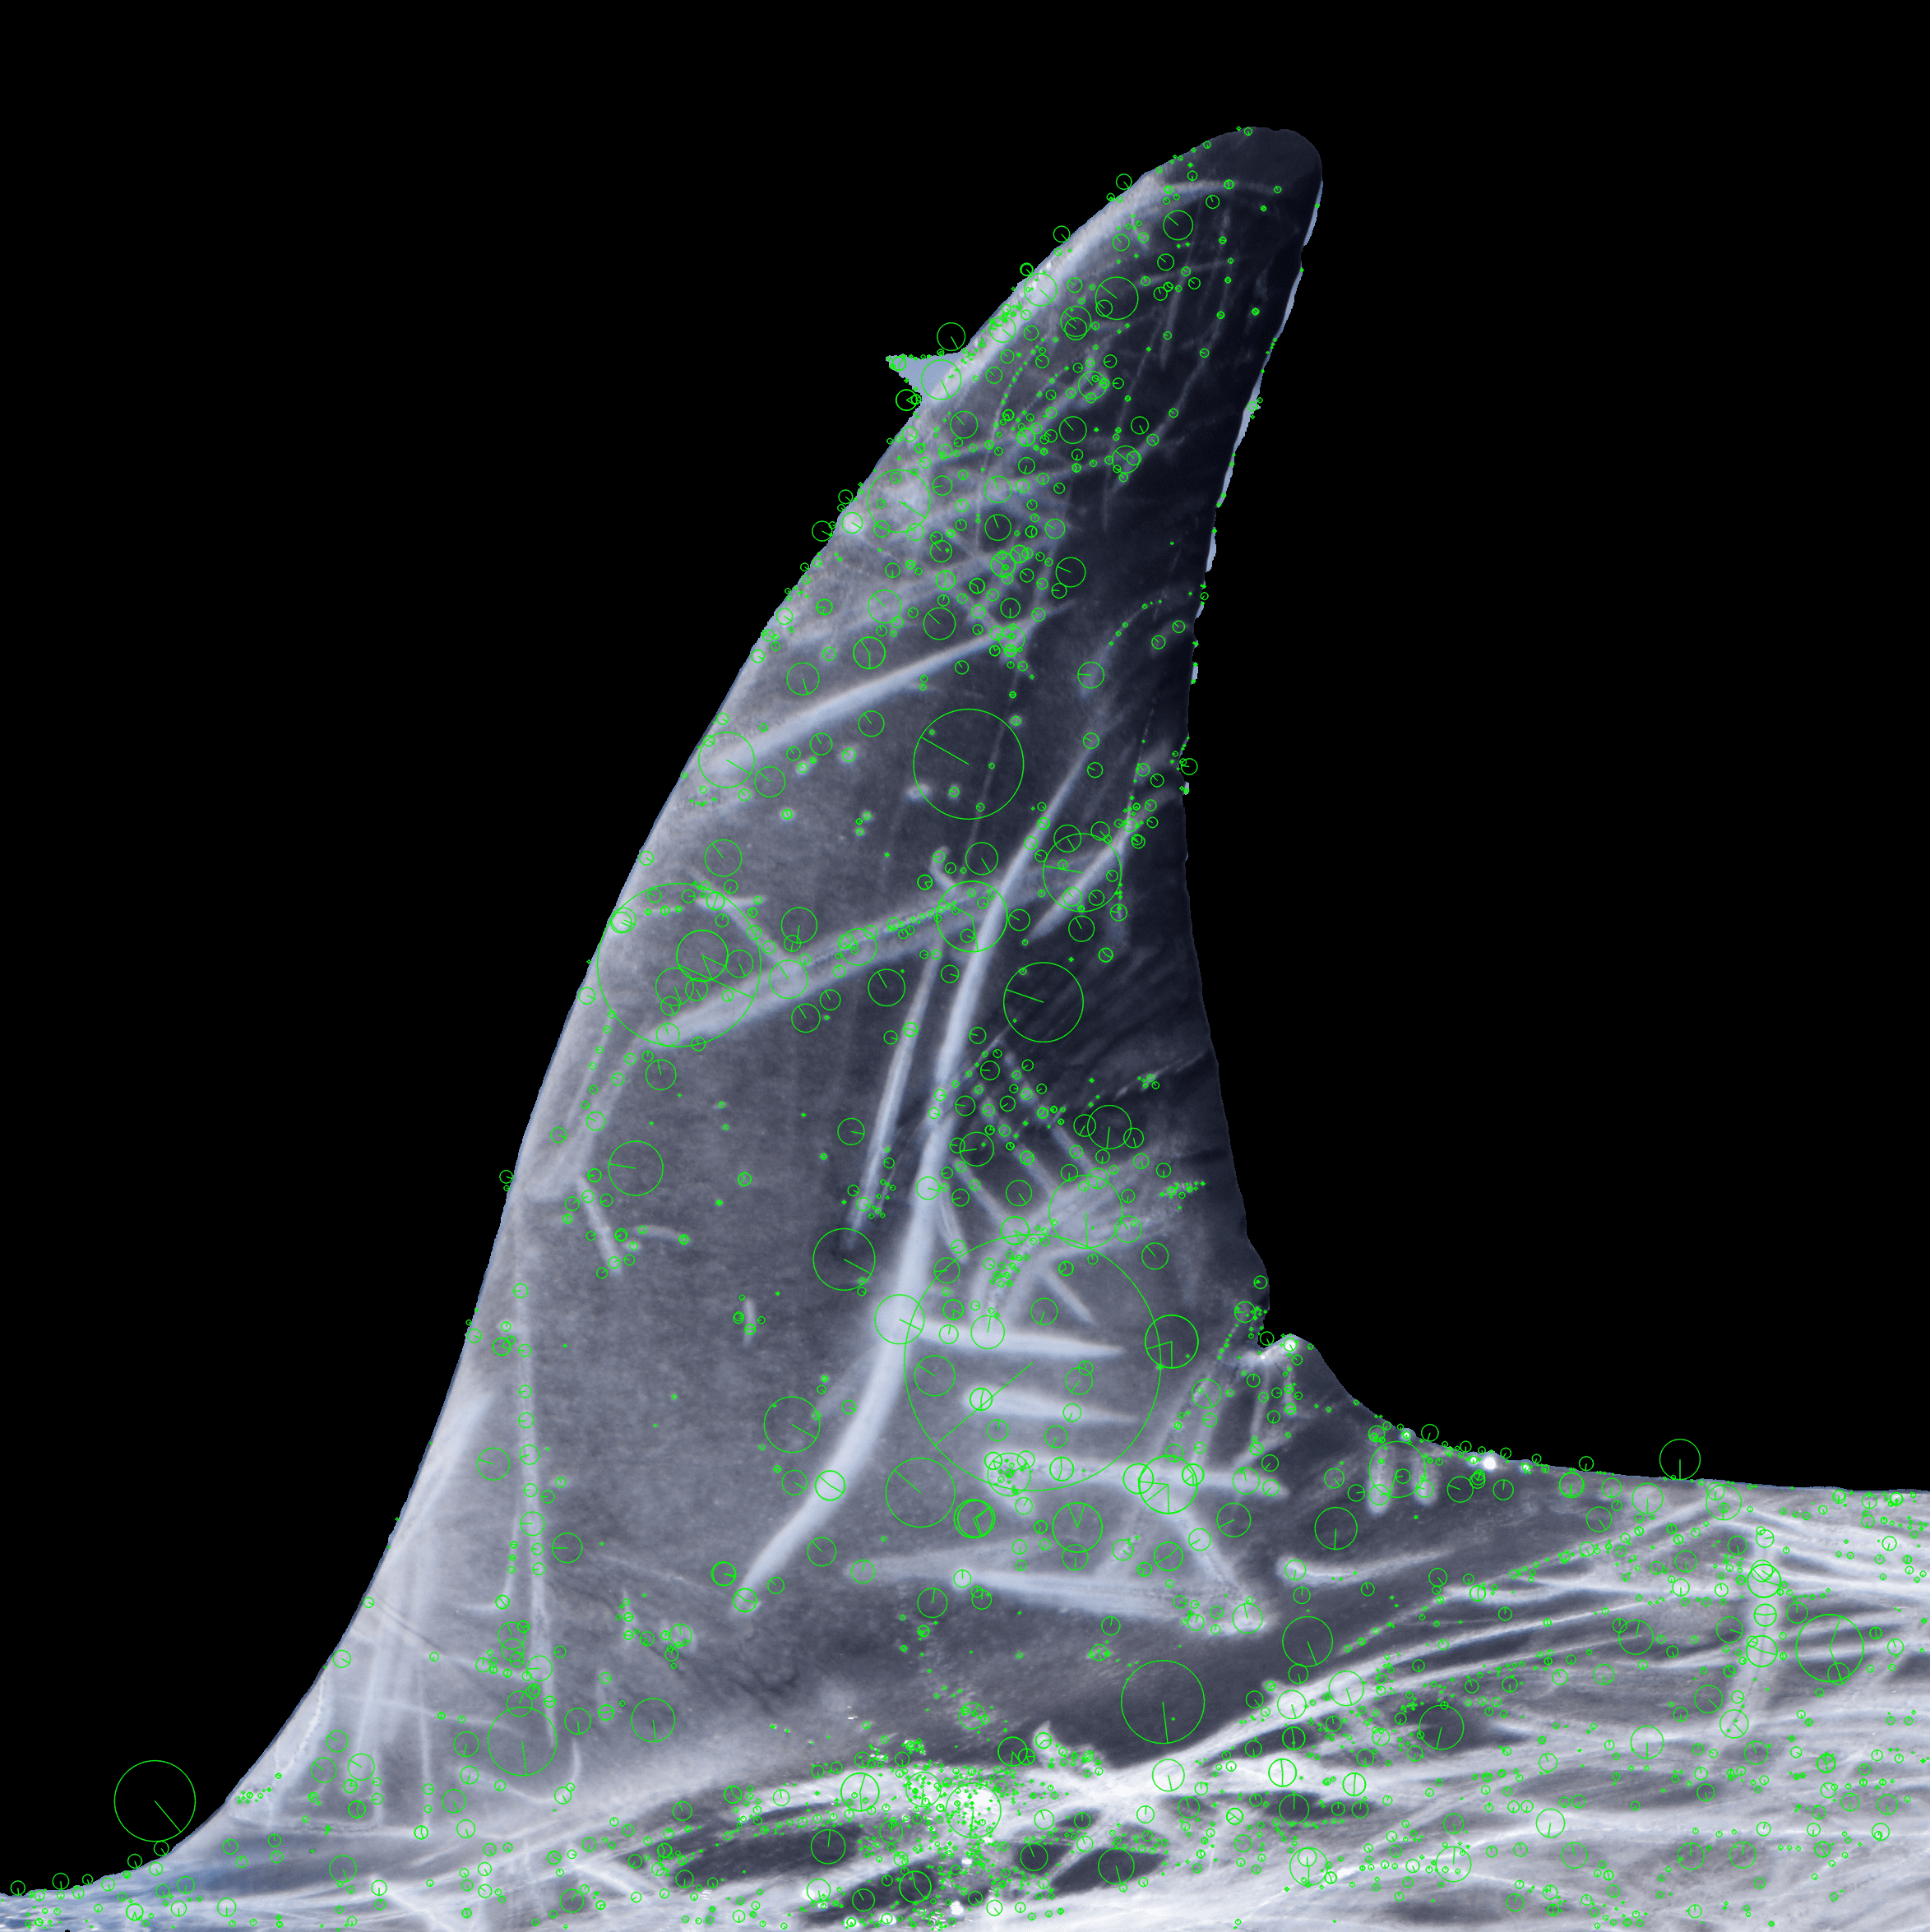
\includegraphics[width=\textwidth]{assets/images/methods/porting/features_extraction/features.png}   
        \caption{Feature estratte}
      \end{minipage}
    \end{figure}
    A questo punto la maschera della pinna del delfino è stata estratta, 
    ora si può passare alla fase di feature extraction, nello specifico l'algoritmo utilizzato 
    è Scale Invariant Feature Transform (SIFT), lo stesso della versione MATLAB,
    anche se nel corso dello sviluppo sono stati testati i seguenti algorimti di feature extraction:
    \begin{itemize}
      \item SIFT (Scale-Invariant Feature Transform \cite{lowe2004distinctive}): L'algoritmo SIFT è ampiamente utilizzato per estrarre feature invarianti rispetto alla scala e alla rotazione. Rileva punti di interesse in un'immagine, calcola le loro descrizioni basate su gradienti di intensità e crea una rappresentazione compatta delle feature. SIFT è noto per la sua robustezza rispetto alle variazioni di scala, rotazione, illuminazione e occlusioni.
      \item ORB (Oriented FAST and Rotated BRIEF \cite{rublee2011orb}): L'algoritmo ORB combina le caratteristiche di rilevazione rapida degli angoli (FAST) e il descrittore binario BRIEF. È un algoritmo efficiente che estrae feature invarianti rispetto alla scala e all'orientazione. ORB utilizza un rilevatore di angoli per individuare punti di interesse, calcola gli orientamenti locali e genera descrittori binari per le feature.
      \newpage
      \item BRISK (Binary Robust Invariant Scalable Keypoints \cite{leutenegger2011brisk}): L'algoritmo BRISK è un metodo basato su descrittori binari che utilizza un rilevatore adattativo di punti di interesse. BRISK calcola un set di punti di interesse utilizzando un rilevatore adattativo basato su una rappresentazione piramidale dell'immagine. Successivamente, calcola i descrittori binari basati su informazioni di intensità e orientazione.
      \item AKAZE (Accelerated-KAZE \cite{alcantarilla2012fast}): L'algoritmo AKAZE è una variante accelerata dell'algoritmo KAZE, che a sua volta si basa sulla rilevazione di blob multiscale e sul calcolo di descrittori basati su regioni. AKAZE è noto per la sua robustezza alle variazioni di scala, rotazione, rumore e cambiamenti di illuminazione.
    \end{itemize}
\begin{lstlisting}
#La pinna estratta viene convertita in scala di grigi
gray_fin = cv2.cvtColor(fin, cv2.COLOR_BGR2GRAY)

#Vengono estratti keypoint e descrittori
#In modo analogo si estraggone le feature con ORB, BRISK e AKAZE
sift = cv2.SIFT_create()
sift_keypoints, sift_descriptors = sift.detectAndCompute(gray_fin, None)

# Calcola la varianza dei descrittori
variances = np.var(sift_descriptors, axis=1)

# Soglia per la varianza per selezionare le feature importanti
variance_threshold = 0.1

# Seleziona solo le feature con varianza superiore alla soglia
selected_indices = np.where(variances > variance_threshold)[0]
sift_keypoints = [sift_keypoints[i] for i in selected_indices]
sift_descriptors = sift_descriptors[selected_indices]
\end{lstlisting}
      L'utilizzo della varianza come criterio per la selezione delle feature si basa su una considerazione matematica fondamentale:
      la varianza misura la dispersione dei dati intorno alla loro media.
      In termini di feature extraction, la varianza può essere utilizzata 
      per valutare quanto le feature variano all'interno di un set di dati.
      Feature con varianza alta indicano una maggiore variabilità dei valori,
      mentre feature con varianza bassa indicano una minore variabilità dei valori.
      L'idea di utilizzare la varianza per selezionare le feature 
      più importanti si basa sul presupposto che le feature più rilevanti 
      per un determinato compito o problema presentano una maggiore variabilità rispetto alle feature meno rilevanti.
      Pertanto, selezionando le feature con una varianza superiore a una soglia specificata, 
      si tende a mantenere le feature che portano informazioni significative.
      \subsection{Salvataggio dataset}
      Il salvataggio delle feature estratte è stato implementato tramite Protocol Buffer (Protocolbuf),
      è un meccanismo di serializzazione dei dati sviluppato da Google.
      È un formato di scambio di dati binario che consente di definire la struttura 
      dei dati in modo dichiarativo utilizzando un file di definizione del protocollo (.proto).
      Questo file di definizione specifica i tipi di dati e i messaggi che possono essere trasmessi utilizzando Protobuf.

      Protobuf offre diverse caratteristiche e vantaggi rispetto ad altri formati di serializzazione dei dati come XML e JSON.
      Alcune delle caratteristiche principali di Protobuf includono:
      \begin{itemize}
        \item Efficienza: I dati serializzati con Protobuf sono più compatti rispetto ad altri formati come JSON o XML, risultando in dimensioni di dati più ridotte. Questo porta a un minor utilizzo dello spazio di archiviazione e una trasmissione più veloce dei dati su una rete.
        \newpage
        \item Velocità: La serializzazione e deserializzazione dei dati utilizzando Protobuf sono molto efficienti e veloci. I dati possono essere facilmente convertiti in un formato binario e viceversa, garantendo prestazioni elevate.
        \item Interoperabilità: I file di definizione del protocollo (.proto) consentono di generare codice sorgente in diverse lingue di programmazione, inclusi C++, Java, Python, Dart e molti altri. Questo facilita l'interoperabilità tra diversi sistemi che utilizzano linguaggi di programmazione diversi.
        \item Tipizzazione forte: Protobuf definisce tipi di dati specifici nel file di definizione del protocollo, consentendo una tipizzazione forte durante la serializzazione e deserializzazione dei dati. Ciò offre un maggiore controllo sui dati trasmessi e contribuisce a ridurre gli errori di interpretazione dei dati.
      \end{itemize}
      \newpage
      \subsection{Match feature}
      Dopo il salvataggio del dataset contenente tutti i keypoint e descrittori 
      \\ per ogni immagine, raggruppati per nome di delfino si è passato ad implementare il match con OpenCV,
      \begin{lstlisting}
bf = cv2.BFMatcher(cv2.NORM_L2, crossCheck=True)

# Match descriptors of the two images
matches: list[cv2.DMatch] = bf.match(dp1, dp2)

# Sort the matches by distance
matches = sorted(matches, key=lambda x: x.distance)

# Set a threshold for selecting good matches

if N > 0:
  matches = matches[:N]

good_matches = [m for m in matches if m.distance < thresh]

match_img = cv2.drawMatches(img1, kp1, img2, kp2, matches, None, flags=cv2.DrawMatchesFlags_NOT_DRAW_SINGLE_POINTS)

      \end{lstlisting}

      \newpage
    \section{Estrazione maschera con Deep Learning}
      Durante lo svilupppo del porting, è nata l'esigenza di creare un dataset
      composto da vere maschere create a mano, per avere un metro di paragone da
      utilizzare con la precedente versione di SPIR per stabilire i progressi fatti nell'estrazione
      delle maschere, proprio questa necessità ha fornito l'idea per lo studio paralello di
      una rete neurale di tipo deep learning, avente l'obiettivo di estrarre le maschere per il 
      ritaglio delle pinne di delfino.
      L'intero sviluppo della rete neurale è stato fatto 
      nell'ambiente virtuale di Google Colab \cite{colab}, grazie ad esso è stato 
      possibile sfruttare GPU e TPU per l'addestramento del modello, andando a velocizzare i tempi.
      \subsection{Dataset}
      \begin{figure}[H]
        \centering
        \begin{minipage}{0.4\textwidth}
          \centering
          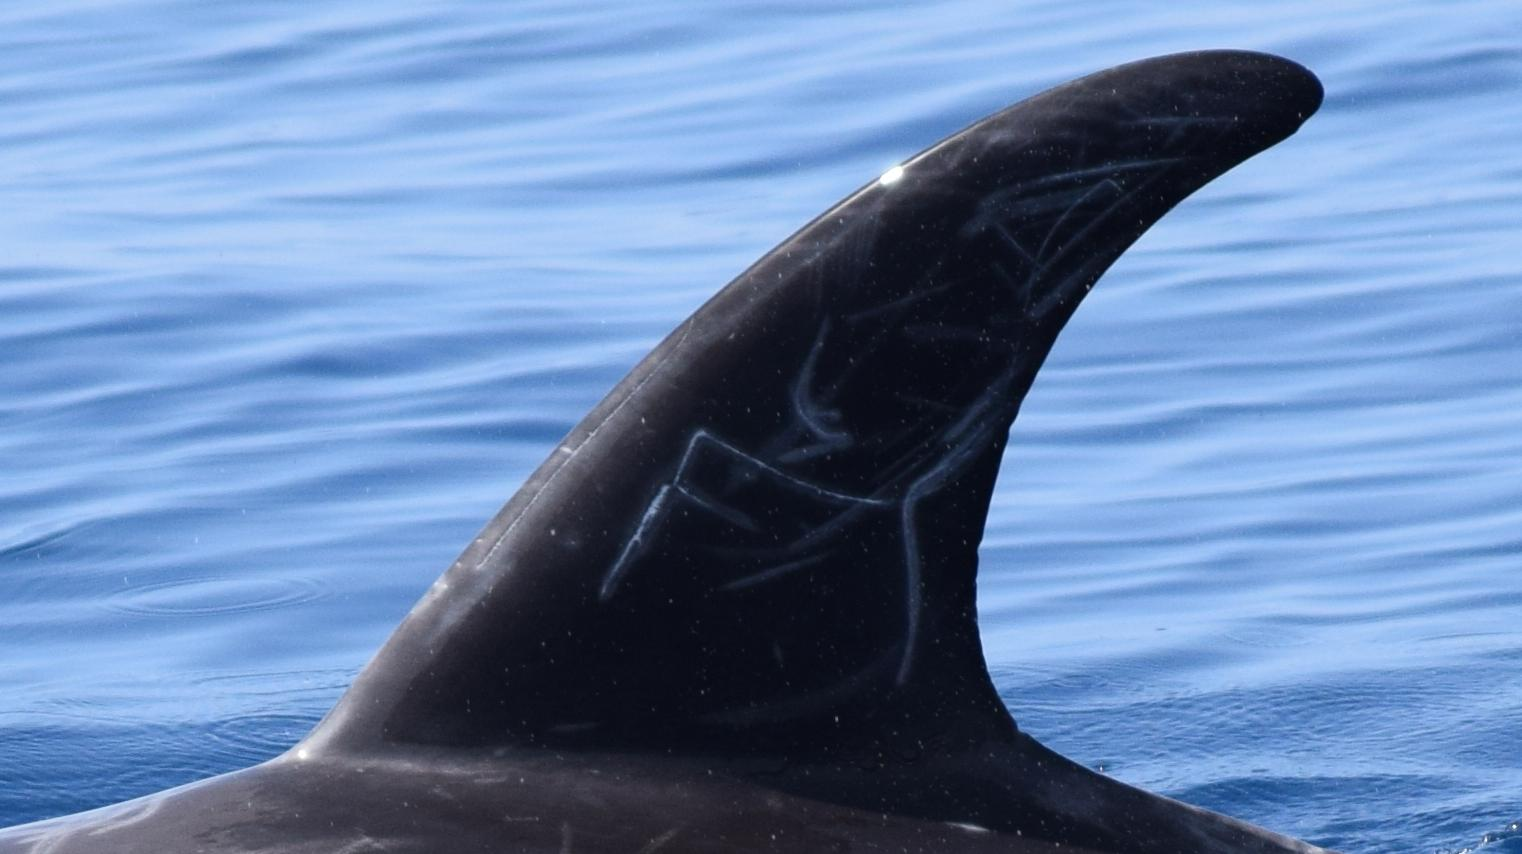
\includegraphics[width=\textwidth]{assets/images/methods/deep/dataset/original.png}   
          \caption{Immagine originale}
        \end{minipage}
        \begin{minipage}{0.4\textwidth}
          \centering
          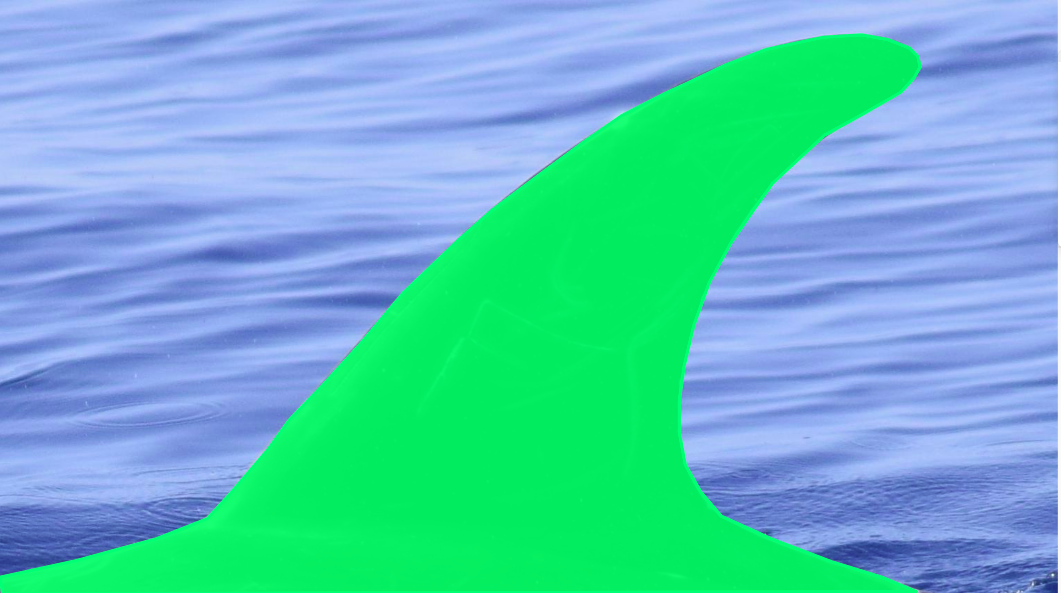
\includegraphics[width=\textwidth]{assets/images/methods/deep/dataset/mask.png}   
          \caption{Maschera poligono}
        \end{minipage}
      \end{figure}
      Il dataset è stato creato utilizzando il software open source Label Studio \cite{labelstudio}, il quale è stato installato su un server
      remoto, ciò ha permesso di accedere facilmente da browser, il software offre due tipi di 
      template per Object Segmentation:
      \begin{itemize}
        \item Maschere: le annotazioni sono rappresentate come maschere binarie che indicano l'area esatta degli oggetti di interesse. Ogni pixel può essere 1 (oggetto) o 0 (sfondo).
        \item Poligoni: le annotazioni sono rappresentate come contorni poligonali che delimitano l'area degli oggetti. Sono definite da una serie di vertici o punti che seguono i contorni degli oggetti.
      \end{itemize}
      In questo caso è stato scelto di utilizzare un dataset basato su label di tipo poligonale,
      questo dettato anche dalla velocità di creazione dei poligoni, un minor costo computazionale 
      di calcolo rispetto a dataset basato su maschere.
      In totale si è lavorato su un dataset di 1725 foto, delle quali per ragioni
      di tempo "solo" 150 sono state descritte con maschere poligonali. 
      Come formato di salvataggio del dataset è stato scelto COCO \cite{coco}, 
      per i seguenti motivi:
      \begin{itemize}
        \item Struttura organizzata: Il formato COCO offre una struttura ben definita per il dataset di segmentazione degli oggetti. Fornisce una gerarchia chiara per le annotazioni, le immagini e le categorie degli oggetti, semplificando l'organizzazione e la gestione dei dati.
        \item Annotazioni precise: COCO consente di annotare gli oggetti di interesse all'interno delle immagini utilizzando maschere o poligoni, permettendo una rappresentazione accurata delle aree degli oggetti. Questo consente di addestrare modelli di segmentazione più precisi e dettagliati.
        \item Metriche di valutazione standard: COCO fornisce metriche di valutazione standard per valutare le prestazioni dei modelli di segmentazione degli oggetti. Questo facilita il confronto tra i diversi approcci e la valutazione delle prestazioni in modo coerente e affidabile.
        \item Ampia comunità e risorse: Il formato COCO è supportato da una vasta comunità di ricercatori e sviluppatori nel campo della visione artificiale. Ciò significa che ci sono molte risorse, strumenti e modelli disponibili per lavorare con il formato COCO, semplificando lo sviluppo e la sperimentazione di nuovi metodi di segmentazione degli oggetti.
      \end{itemize}
      \newpage
      \subsection{Rete}
      Tra le varie alternative disponibili nel panorama delle librerie Python per ML e Deep,
      la scelta è stata guidata dal miglior compromesso in termini di flessibilità e scalabilità,
      anche in vista di sviluppi futuri del codice, questo ha portato a scegliere
      TensorFlow \cite{tensorflow} come libreria, evidenziando i seguenti vantaggi:
      \begin{itemize}
        \item Ampia adozione e supporto della comunità: TensorFlow è uno dei framework di deep learning più popolari ed è ampiamente utilizzato in ambito accademico e industriale. Ciò significa che ci sono molte risorse, documentazione, tutorial e una vasta comunità di sviluppatori pronti a fornire supporto.
        \item Ecosistema completo: TensorFlow fornisce un ecosistema completo per la creazione e la distribuzione di modelli di machine learning. Include strumenti per la pre-elaborazione dei dati, la creazione dei modelli, l'addestramento, l'ottimizzazione e l'inferenza.
        \item Scalabilità e prestazioni: TensorFlow è stato progettato per sfruttare appieno le risorse hardware disponibili, inclusi processori multi-core, GPU e TPU. Questo consente di ottenere prestazioni elevate e di sfruttare al meglio le risorse hardware disponibili.
        \item Supporto multi-piattaforma: TensorFlow è supportato su diverse piattaforme, tra cui desktop, server, dispositivi mobili e dispositivi IoT. Ciò consente di creare modelli una volta e distribuirli su diverse piattaforme senza dover ripensare completamente l'implementazione.
      \end{itemize}
      \newpage
      Avendo il dataset pronto in formato COCO, non è stato difficile passare al
      caricamento e creazione del dataset in TensorFlow, 
      dato che il formato COCO salva i modelli e i relativi label
      in formato JSON è stato necessario creare un metodo per il 
      parsing, da JSON a TFRecord, questo permette di lavorare su 
      un tipo di dataset composto da righe, con anche la possibilità
      di salvare il dataset in diversi file .tfrecord di dimensioni fissate
      così da ottimizzare le operazioni di caricamento del dataset in memoria. 
      \begin{lstlisting}
class Augment(tf.keras.layers.Layer):
  #Viene impostato il seed per avere sempre la stessa generazione
  def __init__(self, seed=42):
    super().__init__()
    self.augment_inputs = tf.keras.layers.RandomFlip(mode="horizontal", seed=seed)
    
    self.augment_inputs_rotation = tf.keras.layers.RandomRotation(factor=0.2, seed=seed)
    
    self.augment_inputs_zoom = tf.keras.layers.RandomZoom(height_factor=(-0.2, 0.2), width_factor=(-0.2, 0.2), seed=seed)
#...
      \end{lstlisting}
 
      Data la scarsa quantità di modelli descritti da poligoni nel dataset (solo 150)
      si è optato per applicare tecniche di data augmentation o aumento di dati tra cui: riflessione, ingrandimento e rotazione,
      queste trasformazioni vengono applicate naturalmente sia al modello (foto del delfino) 
      e sia al poligono che ne descrive la maschera 
      della pinna, la scelta se applicare una delle trasformazioni al modello è fatta in modo 
      casuale dai metodi di TensorFlow (tf.keras.layers).
    
      \begin{figure}[H]
        \centering
        \begin{minipage}{0.8\textwidth}
          \centering
          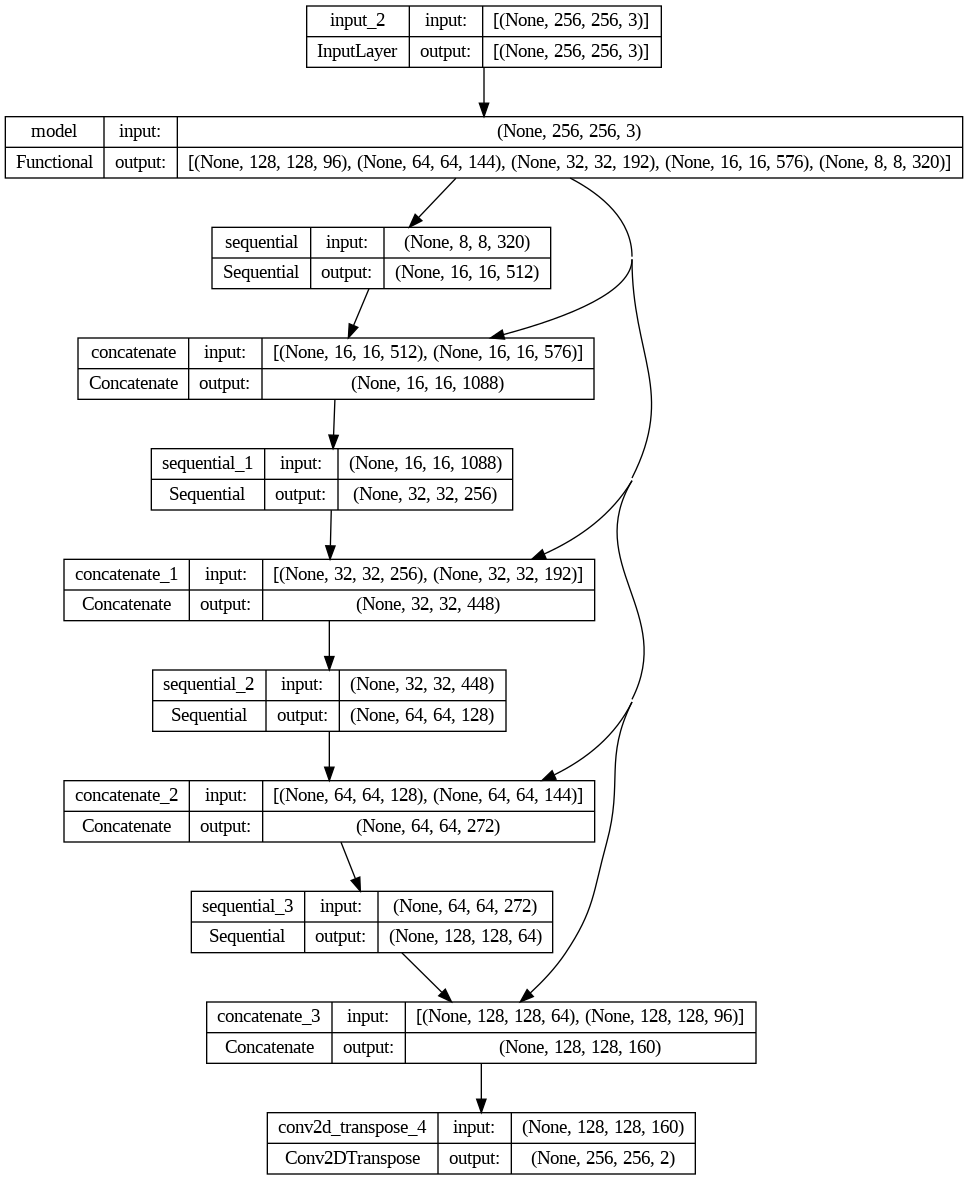
\includegraphics[width=\textwidth]{assets/images/methods/deep/network/network.png}   
          \caption{Struttura rete neurale}
        \end{minipage}
      \end{figure}
      Una volta costruito il dataset in formato TFRecordDataset si può passare
      alla struttura della rete, come modello per effettuare Object Segmentation
      è stato scelto U-Net \cite{ronneberger2015u},
      \\ 
      U-Net è un modello di rete neurale che si è dimostrato efficace per la segmentazione delle immagini,
      compresa la creazione di maschere per oggetti di forma complessa come le pinne di delfino.
      Le caratteristiche chiave di U-Net che lo rendono un buon modello per questo compito sono:

      \begin{itemize}
        \item Architettura a forma di U: U-Net utilizza un'architettura a forma di U, che combina un percorso di contrazione (encoder) con un percorso di espansione (decoder). Questa struttura consente di catturare dettagli a diverse scale e di ricostruire con precisione le forme complesse delle pinne di delfino.
        \item Connessioni skip: U-Net incorpora connessioni skip tra le diverse profondità dell'encoder e del decoder. Queste connessioni consentono di preservare le informazioni a diverse scale spaziali durante il processo di up-sampling, aiutando a ripristinare dettagli fini nelle maschere delle pinne di delfino.
        \item Utilizzo di convoluzioni e pooling: U-Net utilizza convoluzioni e operazioni di pooling per estrarre progressivamente le caratteristiche delle immagini in diverse profondità. Questo aiuta il modello a identificare gli elementi distintivi delle pinne di delfino e a discriminare tra le regioni di interesse e lo sfondo.
        \item Utilizzo di dati di addestramento limitati: U-Net è stato progettato per funzionare bene anche con dataset di addestramento limitati. La sua architettura compatta e le connessioni skip consentono di ottenere buone prestazioni anche con un numero ridotto di esempi di addestramento.
      \end{itemize}

    \section{Backend SPIR}
    dsad
    \section{Frontend SPIR}

\chapter{Risultati sperimentali}
  \section{Valutazione dei risultati}
    \subsection{Confronto tra i diversi approcci implementati}
    \subsection{Analisi delle prestazioni e dei risultati ottenuti}
  \section{Limitazioni e problematiche riscontrate con approccio Deep Learning}

\chapter{Conclusioni}
  \section{Riepilogo degli obiettivi raggiunti}
  \section{Possibili sviluppi futuri}

\chapter{Codice sorgente}
  \section{Implementazione dell'algoritmo SPIR}
  \section{Implementazione della rete neurale U-Net}
  \section{Codice per l'estrazione delle maschere con OpenCV}
  \section{Codice per l'interfaccia utente in Flutter}

  \bibliographystyle{plain}
  \bibliography{bibliography}
\end{document}